%===============================================================================
% LaTeX sjabloon voor de bachelorproef toegepaste informatica aan HOGENT
% Meer info op https://github.com/HoGentTIN/latex-hogent-report
%===============================================================================

\documentclass[dutch,dit,thesis]{hogentreport}

% TODO:
% - If necessary, replace the option `dit`' with your own department!
%   Valid entries are dbo, dbt, dgz, dit, dlo, dog, dsa, soa
% - If you write your thesis in English (remark: only possible after getting
%   explicit approval!), remove the option "dutch," or replace with "english".

\usepackage{lipsum} % For blind text, can be removed after adding actual content

%% Pictures to include in the text can be put in the graphics/ folder
\graphicspath{{../graphics/}}

%% For source code highlighting, requires pygments to be installed
%% Compile with the -shell-escape flag!
%\usepackage[section]{minted}
%% If you compile with the make_thesis.{bat,sh} script, use the following
%% import instead:

\usepackage[section,outputdir=../output]{minted}
\usemintedstyle{solarized-light}
\definecolor{bg}{RGB}{253,246,227} %% Set the background color of the codeframe

%% Change this line to edit the line numbering style:
\renewcommand{\theFancyVerbLine}{\ttfamily\scriptsize\arabic{FancyVerbLine}}

%% Macro definition to load external java source files with \javacode{filename}:
\newmintedfile[javacode]{java}{
    bgcolor=bg,
    fontfamily=tt,
    linenos=true,
    numberblanklines=true,
    numbersep=5pt,
    gobble=0,
    framesep=2mm,
    funcnamehighlighting=true,
    tabsize=4,
    obeytabs=false,
    breaklines=true,
    mathescape=false
    samepage=false,
    showspaces=false,
    showtabs =false,
    texcl=false,
}

% Other packages not already included can be imported here

%%---------- Document metadata -------------------------------------------------
% TODO: Replace this with your own information
\author{Van Achter Levi}
\supervisor{B. Vertonghen}
\cosupervisor{Mr. S. D'Hollander}
\title{Onderzoek naar pentesting binnen een webomgeving}
\academicyear{\advance\year by -1 \the\year--\advance\year by 1 \the\year}
\examperiod{1}
\degreesought{\IfLanguageName{dutch}{Professionele bachelor in de toegepaste informatica}{Bachelor of applied computer science}}
\partialthesis{false} %% To display 'in partial fulfilment'
%\institution{Internshipcompany BVBA.}

%% Add global exceptions to the hyphenation here
\hyphenation{back-slash}

%% The bibliography (style and settings are  found in hogentthesis.cls)
\addbibresource{bachproef.bib}            %% Bibliography file
\addbibresource{../voorstel/voorstel.bib} %% Bibliography research proposal
\defbibheading{bibempty}{}

%% Prevent empty pages for right-handed chapter starts in twoside mode
\renewcommand{\cleardoublepage}{\clearpage}

\renewcommand{\arraystretch}{1.2}

%% Content starts here.
\begin{document}

%---------- Front matter -------------------------------------------------------

\frontmatter

\hypersetup{pageanchor=false} %% Disable page numbering references
%% Render a Dutch outer title page if the main language is English
\IfLanguageName{english}{%
    %% If necessary, information can be changed here
    \degreesought{Professionele Bachelor toegepaste informatica}%
    \begin{otherlanguage}{dutch}%
       \maketitle%
    \end{otherlanguage}%
}{}


%% Generates title page content
\maketitle
\hypersetup{pageanchor=true}

%%=============================================================================
%% Voorwoord
%%=============================================================================

\chapter*{\IfLanguageName{dutch}{Woord vooraf}{Preface}}%
\label{ch:voorwoord}

%% TODO:
%% Het voorwoord is het enige deel van de bachelorproef waar je vanuit je
%% eigen standpunt (``ik-vorm'') mag schrijven. Je kan hier bv. motiveren
%% waarom jij het onderwerp wil bespreken.
%% Vergeet ook niet te bedanken wie je geholpen/gesteund/... heeft

Aan de start van mijn studie Mobile en Enterprise Development was ik mij snel bewust van het belang van cybersecurity in de wereld van softwareontwikkeling. 
Veiligheid wordt steeds relevanter binnen onze samenleving en het is cruciaal dat dit element hand in hand gaat met de ontwikkeling van technologie. 
Met deze context in gedachten koos ik voor mijn bachelorproef een onderwerp dat niet alleen mijn passie in softwareontwikkeling combineert met cybersecurity, 
maar eveneens een essentieel topic in de huidige technologiewereld: het evalueren van de effectiviteit en gebruiksvriendelijkheid van 
penetratietesttools binnen diverse webomgevingen.

Mijn keuze werd verder gedreven door de overtuiging dat een grondige kennis van cybersecurity belangrijk is om mijn vaardigheden als ontwikkelaar naar een hoger niveau te tillen. In het huidige 
tijdperk raken technologische systemen steeds meer verweven met alle aspecten van ons dagelijks leven. Het is daarom cruciaal dat deze systemen niet alleen 
functioneel en efficiënt zijn, maar ook veilig en betrouwbaar. Het besef dat de veiligheid van software daardoor niet alleen de verantwoordelijkheid 
is van security experts, maar van alle IT-professionals, waaronder ontwikkelaars, versterkt enkel nog deze keuze..

Gedurende mijn onderzoek heb ik waardevolle inzichten verkregen hoe verschillende tools presteren in termen van detectie van kwetsbaarheden en de 
gebruiksvriendelijkheid ervan binnen diverse webomgevingen. Dit onderzoek heeft niet alleen mijn kennis en vaardigheden 
verrijkt, maar tevens mijn waardering voor de complexiteit van pentesting tools en het nut ervan voor de beveiliging in softwareontwikkeling versterkt.

Ik wil in dit voorwoord het bedrijf Sinregio en in het bijzonder mijn co-promotor bedanken, Stijn D'Hollander, danken voor zijn bereidheid om te helpen en ondersteuning te bieden  
tijdens dit project. Uiteraard dank ik ook meneer Vertonghen, die als begeleider bereid was om sturing en vorming te 
bieden aan deze bachelorproef. Hun bereidheid om inzichten en constructieve feedback te verschaffen, heeft sterk bijgedragen aan het verbreden en uitdiepen van mijn onderzoek.
Verder wil ik mijn familie bedanken voor hun onvoorwaardelijke steun en geduld gedurende mijn hele studie, niet in het minst tijdens de laatste, 
vaak stressvolle fase. Tot slot wil ik mijn stageplaats, 24Flow, bedanken voor hun hulp en ondersteuning wanneer nodig.

Ik hoop dan ook dat mijn werk bijdraagt aan een groter bewustzijn van het belang van cybersecurity in alle lagen van softwareontwikkeling. 
Moge het lezers inspireren om beveiliging als een noodzakelijke pijler van technologische ontwikkeling te omarmen.


Levi Van Achter

Opdorp, 24 mei 2024

%%=============================================================================
%% Samenvatting
%%=============================================================================

% TODO: De "abstract" of samenvatting is een kernachtige (~ 1 blz. voor een
% thesis) synthese van het document.
%
% Een goede abstract biedt een kernachtig antwoord op volgende vragen:
%
% 1. Waarover gaat de bachelorproef?
% 2. Waarom heb je er over geschreven?
% 3. Hoe heb je het onderzoek uitgevoerd?
% 4. Wat waren de resultaten? Wat blijkt uit je onderzoek?
% 5. Wat betekenen je resultaten? Wat is de relevantie voor het werkveld?
%
% Daarom bestaat een abstract uit volgende componenten:
%
% - inleiding + kaderen thema
% - probleemstelling
% - (centrale) onderzoeksvraag
% - onderzoeksdoelstelling
% - methodologie
% - resultaten (beperk tot de belangrijkste, relevant voor de onderzoeksvraag)
% - conclusies, aanbevelingen, beperkingen
%
% LET OP! Een samenvatting is GEEN voorwoord!

%%---------- Nederlandse samenvatting -----------------------------------------
%
% TODO: Als je je bachelorproef in het Engels schrijft, moet je eerst een
% Nederlandse samenvatting invoegen. Haal daarvoor onderstaande code uit
% commentaar.
% Wie zijn bachelorproef in het Nederlands schrijft, kan dit negeren, de inhoud
% wordt niet in het document ingevoegd.

\IfLanguageName{english}{%
\selectlanguage{dutch}
\chapter*{Samenvatting}
\lipsum[1-4]
\selectlanguage{english}
}{}

%%---------- Samenvatting -----------------------------------------------------
% De samenvatting in de hoofdtaal van het document

\chapter*{\IfLanguageName{dutch}{Samenvatting}{Abstract}}

Deze bachelorproef onderzoekt de effectiviteit en gebruiksvriendelijkheid van verschillende penetratietesttools in drie specifieke webomgevingen: 
een WordPress-omgeving zonder beveiligingsplugins, een WordPress-omgeving met beveiligingsplugins, en een Laravel-applicatie. Het onderzoek richt 
zich op het belang van cybersecurity binnen de softwareontwikkeling.

De keuze voor dit onderwerp is ingegeven door de groeiende behoefte aan robuuste beveiligingsmaatregelen in softwareontwikkeling, een cruciaal 
aspect dat vaak onderbelicht blijft in de snelle evolutie van technologische innovaties. Gezien mijn achtergrond in Mobile en Enterprise 
Development, vormde de integratie van cybersecurity in ontwikkelpraktijken een natuurlijke en relevante focus voor mijn studie.

Het onderzoek werd uitgevoerd door middel van een reeks gestructureerde penetratietests, waarbij elke omgeving werd geëvalueerd op 
kwetsbaarheden met behulp van penetratietesttools met name Burp Suite, OWASP ZAP, en Metasploit. De gebruiksvriendelijkheid 
van deze tools werd ook kritisch beoordeeld, om inzicht te bieden in hoe toegankelijk deze tools zijn voor professionals in verschillende 
niveau's van hun cybersecurity-vaardigheden.

De resultaten tonen aan dat de WordPress-omgeving zonder beveiligingsplugins aanzienlijk kwetsbaarder is voor cyberaanvallen, met name 
brute force aanvallen, in vergelijking met de omgevingen waar beveiligingsplugins zijn geïmplementeerd. De Laravel-applicatie toonde 
de hoogste weerstand tegen aanvallen, wat de geavanceerde, ingebouwde beveiligingsmaatregelen van dit framework onderstreept.
Deze uitkomst lag in lijn met de verwachtingen omdat het onderzoekend deel van de studie snel duidelijk maakte hoeveel veiliger 
de security plugin wordfence in wordpress de site maakt.
Bovendien bleek uit de evaluatie dat tools zoals Burp Suite en OWASP ZAP bijzonder gebruiksvriendelijk zijn, terwijl Metasploit 
uitblinkt in zijn uitgebreide functionaliteiten voor diepgaandere penetratietests.

Deze bevindingen zijn van grote waarde voor het werkveld, omdat ze de noodzaak onderstrepen voor het integreren van effectieve 
beveiligingsstrategieën in de ontwikkelingsfase van softwareprojecten. Voor organisaties in het domein van Mobile en Enterprise 
Development suggereren de resultaten dat een investering in goede beveiligingspraktijken en tools niet alleen de veiligheid 
verbetert, maar ook de algehele kwaliteit van de ontwikkelde applicaties. Ook wijst deze studie erop hoe moeilijk het 
is om als software developer zelf pentestings uit te voeren.

Concluderend biedt dit onderzoek praktische aanbevelingen voor de selectie en implementatie van penetratietesttools, met 
nadruk op de combinatie van gebruiksvriendelijkheid en uitgebreide testcapaciteiten om een optimale beveiliging te 
garanderen. De studie benadrukt ook het belang van voortdurende educatie en aanpassing van beveiligingspraktijken aan nieuwe 
bedreigingen, wat essentieel is voor het behouden van een veilige en betrouwbare softwareontwikkelingsomgeving.


%---------- Inhoud, lijst figuren, ... -----------------------------------------

\tableofcontents

% In a list of figures, the complete caption will be included. To prevent this,
% ALWAYS add a short description in the caption!
%
%  \caption[short description]{elaborate description}
%
% If you do, only the short description will be used in the list of figures

\listoffigures

% If you included tables and/or source code listings, uncomment the appropriate
% lines.
%\listoftables
%\listoflistings

% Als je een lijst van afkortingen of termen wil toevoegen, dan hoort die
% hier thuis. Gebruik bijvoorbeeld de ``glossaries'' package.
% https://www.overleaf.com/learn/latex/Glossaries

%---------- Kern ---------------------------------------------------------------

\mainmatter{}

% De eerste hoofdstukken van een bachelorproef zijn meestal een inleiding op
% het onderwerp, literatuurstudie en verantwoording methodologie.
% Aarzel niet om een meer beschrijvende titel aan deze hoofdstukken te geven of
% om bijvoorbeeld de inleiding en/of stand van zaken over meerdere hoofdstukken
% te verspreiden!

%%=============================================================================
%% Inleiding
%%=============================================================================

\chapter{\IfLanguageName{dutch}{Inleiding}{Introduction}}%
\label{ch:inleiding}
Cyberbeveiliging speelt een cruciale rol binnen de bescherming van gevoelige informatie. Het is dan ook essentieel dat organisaties 
effectieve beveiligingstools implementeren om hun webomgevingen te beschermen. Penetratietesten of pentests, zijn  
methodieken om de beveiliging van webapplicaties te beoordelen door ze bloot te stellen aan gesimuleerde 
cyberaanvallen die zich focussen op het onthullen van kwetsbaarheden. Dit onderzoek gaat dieper in op de kwetsbaarheden van deze omgevingen. Het doel is om te bepalen welke tools 
het meest effectief zijn in specifieke situaties en hoe beveiligingsstrategieën aangepast kunnen worden om optimale 
bescherming te bieden.


\section{\IfLanguageName{dutch}{Probleemstelling}{Problem Statement}}%
\label{sec:probleemstelling}

\begin{figure}
  \centering
  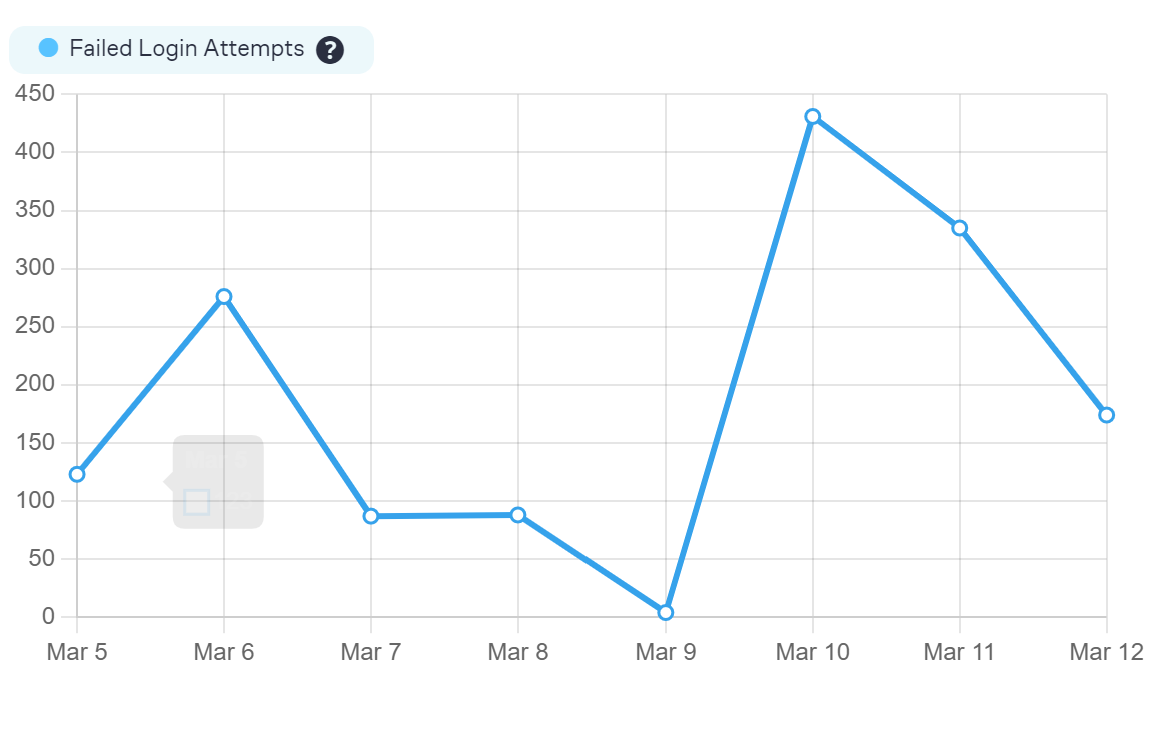
\includegraphics[height=0.3\textheight]{failed_login_attemps_24flow.png}
  \caption[Aantal foutieve logins op de Wordpress website van 24Flow per dag ]{Aantal foutieve logins op de Wordpress website van 24Flow per dag }
\end{figure}
Kleine tot middelgrote IT-servicebedrijven, zoals Sinergio (promotor van dit eindwerk) en 24Flow (stageplaats), worden net 
als elk ander bedrijf dagelijks geconfronteerd met de uitdaging om hun 
webapplicaties alsmaar beter te beschermen tegen cyberaanvallen. Deze bedrijven maken vaak gebruik van populaire webontwikkelingsplatformen 
zoals het CMS WordPress of het ontwikkelingsframework Laravel, die elk op zich unieke en specifieke beveiligingsrisico's en 
kwetsbaarheden kennen. De bescherming van deze platformen wordt dan toevertrouwd aan de implementatie van beveiligingsplugins 
en -tools, waarvan de effectiviteit varieert.

Deze bachelorproef focust zich voornamelijk op het onderzoek naar de effectiviteit van een aantal gangbare penetratietesttools  
bij het identificeren van kwetsbaarheden binnen drie specifieke webomgevingen: een WordPress applicatie zonder beveiligingsplugins,
een WordPress applicatie met beveiligingsplugins en een afgewerkte Laravel applicatie. 

Het doel van dit onderzoek is tweeledig. 
Ten eerste, het vaststellen welke penetratietesttool(s) het meest functioneel zijn aan de hand van objectieve criteria binnen het kader van deze webomgevingen. Ten tweede, 
een analyse maken van de beveiligingsrisico's geassocieerd met elk van de te onderzoeken omgevingen om de vraag te beantwoorden hoe 
veilig of onveilig deze zijn.

De directe doelgroep voor deze bachelorproef is het bedrijf Sinergio, een kleinere IT-serviceprovider die  
werkt met WordPress en Laravel bij het ontwikkelen van websites of webapplicaties voor hun klanten. De resultaten van dit 
onderzoek biedt Sinergio dan ook waardevolle inzichten in de meest doeltreffende manieren om hun webontwikkelingsprojecten beter 
te beveiligen en geeft hun een idee hoe belangrijk het is om beveiligingsplugins te integreren binnen Wordpress-applicaties. 
Dit stelt hen bovendien in staat om onderbouwde beslissingen te nemen over het gebruik van 
beveiligingsstrategieën en -tools. Sinergio zal desgevallend kunnen achterhalen welke pentesting tool het interessantst is 
binnen hun specifieke omgevingen en zal hierdoor in de toekomst dit aspect minder zelf moeten onderzoeken.
Bovendien draagt dit onderzoek bij aan een bredere kennisbasis over webapplicatiebeveiliging, 
wat van belang kan zijn voor andere kleine tot middelgrote IT-bedrijven die vergelijkbare technologieën gebruiken.

\section{\IfLanguageName{dutch}{Onderzoeksvraag}{Research question}}%
\label{sec:onderzoeksvraag}
De onderzoeksvraag wordt opgesplitst in twee luiken.
\begin{enumerate}
  \item Welke penetratietesttool(s) zijn volgens de vooraf bepaalde criteria het meest effectief/efficiënt in het identificeren van kwetsbaarheden in drie specifieke webomgevingen?
  \item Welke specifieke kwetsbaarheden detecteren de penetratietesttools in een WordPress-omgeving zonder beveiligingsplugins en hoe verschilt dit van de omgevingen met beveiligingsplugins en de Laravel-applicatie? 
\end{enumerate}
Deze onderzoeksvragen vormen een duidelijke basis om de werking van de verschillende penetratietesttools te kunnen evalueren 
en om de impact op de geteste webomgevingen op een gestrucureerde manier te kunnen vergelijken. Door de prestaties van de 
tools te beoordelen op vlak van efficiëntie, functionaliteiten, kostprijzen, resourceverbruik, ondersteuning van de community en gebruiksgemak, 
kan dit onderzoek waardevolle inzichten bieden. hierna wordt er gekeken naar de opninie van derden over de tools aan de hand van 
reviews en ervaringen van andere gebruikers.

\section{\IfLanguageName{dutch}{Onderzoeksdoelstelling}{Research objective}}%
\label{sec:onderzoeksdoelstelling}
De doelstelling van deze paper is het uitvoeren van een vergelijkende studie, die de effectiviteit en andere aspecten uit bovenstaand hoofdstuk 
test van verschillende penetratietesttools bij het identificeren van kwetsbaarheden in verschillende webomgevingen.
Het beoogde resultaat is een verslag met gedetailleerde aanbevelingen over de meest aangewezen tool voor de drie geteste 
omgevingen. Het succes werd gemeten aan de hand van de volledigheid van de verzamelde data, de analytische diepgang van de bevindingen 
en de duidelijkheid van de vergelijkende analyse tussen de tools en omgevingen. Dit verslag kan op die manier interessante inzichten bieden die 
bijdragen aan betere beveiligingsstrategieën en -implementaties in webontwikkelingsprojecten.
\section{\IfLanguageName{dutch}{Opzet van deze bachelorproef}{Structure of this bachelor thesis}}%
\label{sec:opzet-bachelorproef}

% Het is gebruikelijk aan het einde van de inleiding een overzicht te
% geven van de opbouw van de rest van de tekst. Deze sectie bevat al een aanzet
% die je kan aanvullen/aanpassen in functie van je eigen tekst.

In het verdere verloop van deze bacheloorproef komen onderstaande hoofdstukken aan bod.

Hoofdstuk~\ref{ch:stand-van-zaken} geeft een overzicht van de stand van zaken binnen het onderzoeksdomein, op basis van een literatuurstudie.

Hoofdstuk~\ref{ch:methodologie} geeft toelichting omtrent de methodologie en de gebruikte onderzoekstechnieken die een antwoord kunnen formuleren op de onderzoeksvragen.

% TODO: Vul hier aan voor je eigen hoofstukken, één of twee zinnen per hoofdstuk
Hoofdstuk~\ref{ch:resultaten} bevat de resultaten van het onderzoek.

Hoofdstuk~\ref{ch:conclusie} bevat de conclusies en hier wordt tevens een antwoord geformuleerd op de onderzoeksvragen. Daarbij wordt overigens ook een aanzet gegeven voor toekomstig onderzoek binnen dit domein.
\chapter{\IfLanguageName{dutch}{Stand van zaken}{State of the art}}%
\label{ch:stand-van-zaken}

% Tip: Begin elk hoofdstuk met een paragraaf inleiding die beschrijft hoe
% dit hoofdstuk past binnen het geheel van de bachelorproef. Geef in het
% bijzonder aan wat de link is met het vorige en volgende hoofdstuk.

% Pas na deze inleidende paragraaf komt de eerste sectiehoofding.
\section{\IfLanguageName{dutch}{Doel van het onderzoek}{Goal of the study}}

Het hoofddoel van dit onderzoek is een grondige evaluatie van de effectiviteit van verschillende penetratietesttools in twee typen webomgevingen: 
een wordPress sites en een op maat gemaakte Laravel applicatie. Deze evaluatie 
heeft tot doel de sterke en zwakke punten van elke pentest tool te identificeren in hun vermogen om kwetsbaarheden te detecteren en weerstand te bieden 
tegen cyberdreigingen. Daarnaast wordt ook de invloed van de structuur van de webomgeving op de prestaties van deze tools onderzocht.
Dit onderzoek maakt gebruik van inzichten uit een recente publicatie in MDPI Electronics, die een uitgebreide analyse van cybersecuritydreigingen en 
de effectiviteit van verschillende verdedigingsmechanismen binnen webapplicaties biedt. Een bijkomend doel is dan ook om de kennis over hoe webapplicaties beter 
beschermd kunnen worden tegen geavanceerde cyberaanvallen uit te diepen. Dit artikel benadrukt specifiek het belang van voortdurende vernieuwing 
in beveiligingsstrategieën om voldoende in te kunnen spelen op de snel evoluerende cyberdreigingen, wat direct gepaard gaat met de doelstellingen van dit 
onderzoek ~\autocite{Altulaihan2023}.

\section{\IfLanguageName{dutch}{Pentesting}{Pentesting}}
\label{sec:pentesting}
Penetration testing (pentesting) vormt een cruciaal onderdeel bij het waarborgen van netwerk-, systeem- en applicatiebeveiliging. 
Wetenschappelijke studies tonen aan dat het proces van pentesting verschillende methodieken omvat, zoals white box, 
black box, en grey box, elk met hun eigen aanpak van kwetsbaarheden in een systeem. Het doel van pentesting is om 
veiligheidszwakheden te identificeren en te exploiteren\footnote{het proces waarbij een tester actief gebruikmaakt 
van veiligheidszwakheden of kwetsbaarheden in een systeem om te laten zien hoe een kwaadwillende aanvaller deze kan misbruiken.} 
om organisaties te helpen begrijpen waar beveiligingskwestbaarheden zich bevinden ~\autocite{Alhamed2023}.

Tijdens de voorbereidingsfase wordt Nmap gebruikt om de netwerkstructuren te verkennen en de actieve hosts en 
services te identificeren. Dit helpt bij het vaststellen van de scope en de doelstellingen van de penetratietest 
door het aanvalsoppervlak duidelijk te maken. Vervolgens vindt in de uitvoeringsfase de test plaats, waarbij tools en methoden worden 
toegepast om kwetsbaarheden te identificeren. Nessus wordt ingezet om diepgaande scans uit te voeren en 
bekende kwetsbaarheden in het netwerk en op systemen te vinden. Metasploit wordt vervolgens gebruikt om deze 
kwetsbaarheden te exploiteren. Hiermee testen de testers of ze daadwerkelijk toegang kunnen krijgen tot 
systemen of data, en bepalen ze de impact van mogelijke beveiligingslekken. Ten slotte worden in de analyse-fase de resultaten 
geanalyseerd en gerapporteerd, inclusief aanbevelingen voor het verbeteren van de beveiliging. De 
informatie verzameld met Metasploit en Nessus speelt een cruciale rol in het begrijpen van de ernst en de 
exploitatie van de geïdentificeerde kwetsbaarheden ~\autocite{Sarker2023}.

Bij het selecteren van tools en methoden voor penetratietests moet rekening worden gehouden met verschillende factoren, zoals de 
grootte van het netwerk, het soort infrastructuur en het type kwetsbaarheden die worden getest. Wetenschappelijke studies 
benadrukken het belang van een grondige planning en voorbereiding om ervoor te zorgen dat een test nauwkeurig en doeltreffend 
wordt uitgevoerd ~\autocite{Alhamed2023}.

Een andere overweging bij penetratietests is het volgen van specifieke normen en richtlijnen, zoals ISO 27000, die ethische 
aspecten en best practices voor pentesting benadrukken ~\autocite{DalalanaBertoglio2017}. Recente ontwikkelingen in technologie, zoals deep 
reinforcement learning\footnote{Bij deep reinforcement learning combineren we de patroonherkenning van deep learning en neurale 
netwerken met het feedback-gebaseerde leren van versterkend leren. Zo kunnen computers intelligente beslissingen nemen en complexe 
taken uitvoeren door te leren van hun interacties met de omgeving}, bieden geavanceerde benaderingen voor automatische pentesting. 
Deze nieuwe methoden kunnen de efficiëntie van het proces verhogen en bijdragen aan een betere detectie van kwetsbaarheden 
~\autocite{Yi2023}.

Voor gedetailleerde informatie en diepgaande analyses van penetratietests in verschillende contexten kunnen wetenschappelijke 
artikelen en studies worden geraadpleegd, die het onderwerp uitvoerig behandelen ~\autocite{Sarker2023}.

\section{\IfLanguageName{dutch}{Webomgevingen}{Web environments}}
\label{sec:Webomgevingen}

\subsection{\IfLanguageName{dutch}{Veiligheidskwetsbaarheden in webapplicaties}{Security vulnerabilities in web applications}}
\label{sec:Veiligheidskwetsbaarheden in Webomgevingen}
\begin{figure}
    \centering
    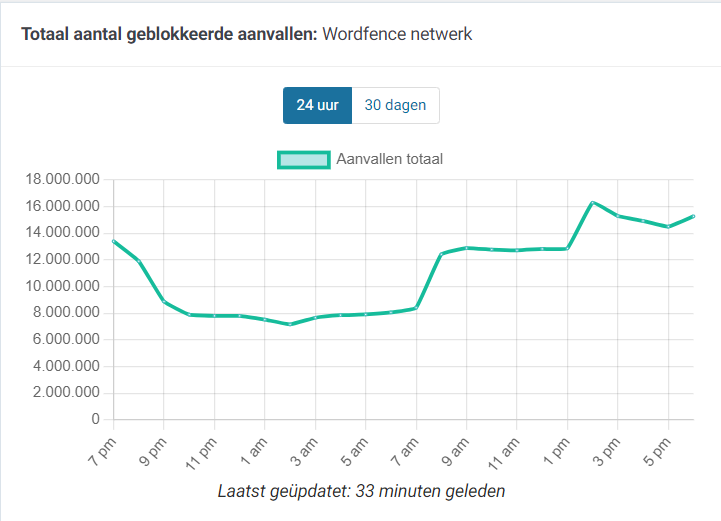
\includegraphics[height=0.3\textheight]{wordfence_stopped_attacks.png}
    \caption[Totaal aantal geblokkeerde aanvallen: Wordfence netwerk]{Totaal aantal geblokkeerde aanvallen: Wordfence netwerk}
    \label{fig:stopped_attacks}
\end{figure}

In de methodologie bij het testen van webomgevingen met name CMS WordPress en php framework Laravel, speelt het identificeren van veelvoorkomende 
kwetsbaarheden een belangrijke rol. Zoals hiervoor aangehaald valt het onderzoeken van kwetsbaarheden in webapplicaties onder 
de fase voorbereiding van een pentest.

In een WordPress omgeving zonder beveiligingsplugins moeten misconfiguraties zoals onbeschermde back-ups 
en tijdelijke bestanden worden geïdentificeerd, omdat ze gevoelige informatie kunnen lekken. Deze onbeschermde bestanden kunnen 
ertoe leiden dat een aanvaller toegang krijgt tot gevoelige informatie, zoals database-informatie in het geval van 
wp-config.php-bestanden\footnote{een bestand dat over zeer belangrijke informatie over een website beschikt} 
~\autocite{DalalanaBertoglio2017}.

Bij het testen van WordPress met beveiligingsplugin(s) is het belangrijk om de effectiviteit van beveiligingsmaatregelen te 
evalueren. Op figuur \ref{fig:stopped_attacks} kan er gezien worden hoeveel aanvallen het wordfence netwerk per dag tegenhoudt. Kwetsbaarheden 
zoals SQL-injecties en Cross-Site Scripting (XSS) zijn belangrijke aandachtsgebieden voor pentesters, vooral in WordPress-omgevingen 
met up-to-date beveiligingsplugin(s) ~\autocite{Albahar2022}.

Bij Laravel-applicaties is het belangrijk om te letten op backend-logica, authenticatie en sessiebeheer. 
Mass assignment-kwetsbaarheden moeten zorgvuldig worden onderzocht om ongeautoriseerde gegevenswijzigingen te voorkomen.
Mass assignment is een techniek binnen Eloquent de Object-Relational Mapper\footnote{een manier om programmeercode af 
te stemmen op databasestructuren} (ORM) van Laravel  waarbij een gebruiker meerdere velden tegelijk kan bijwerken, wat een beveiligingsrisico kan vormen. 
Daarnaast is het essentieel om te testen op SQL-injecties en te zorgen voor veilige authenticatie in Laravel-applicaties 
~\autocite{Altulaihan2023}.

Een effectieve methodologie omvat een grondige beoordeling van de infrastructuur, identificatie van kwetsbaarheden en het 
testen van beveiligingsmaatregelen met diverse tools zoals Metasploit, Burp Suite en OWASP ZAP ~\autocite{Ravindran2022}. 
Het uiteindelijke doel is om kwetsbaarheden te ontdekken en effectieve maatregelen te nemen om de beveiliging van webomgevingen 
te versterken.

\subsection{\IfLanguageName{dutch}{Aanvallen op veiligheidskwetsbaarheden in webapplicaties}{Attacks on Security vulnerabilities in web applications}}
\label{sec:Veiligheidskwetsbaarheden in Webomgevingen}
In de dynamische wereld van webbeveiliging biedt het Open Web Application Security Project (OWASP) de bekendste richtlijnen en hulpmiddelen om te vechten 
tegen de voortdurende dreiging van cyberaanvallen. OWASP, een internationale non-profit organisatie, speelt een cruciale rol door het bevorderen van 
veiligere softwarepraktijken. Ze zijn het meest bekend voor hun publicatie van de OWASP Top 10, een lijst die de tien meest kritieke veiligheidsrisico's 
voor webapplicaties benadrukt. Deze lijst wordt breed erkend en gerespecteerd in de cybersecurity gemeenschap en dient als een fundamentele leidraad 
voor ontwikkelaars en beveiligingsexperts wereldwijd. Door de complexiteit van moderne webapplicaties te adresseren en praktische adviezen voor 
beperkingen en preventie te bieden, helpt OWASP organisaties om hun digitale assets effectiever te beschermen tegen bedreigingen zoals SQL-injectie, 
Cross-Site Scripting (XSS), en andere gevaarlijke kwetsbaarheden ~\autocite{Priyawati2022}.
\begin{figure}
    \centering
    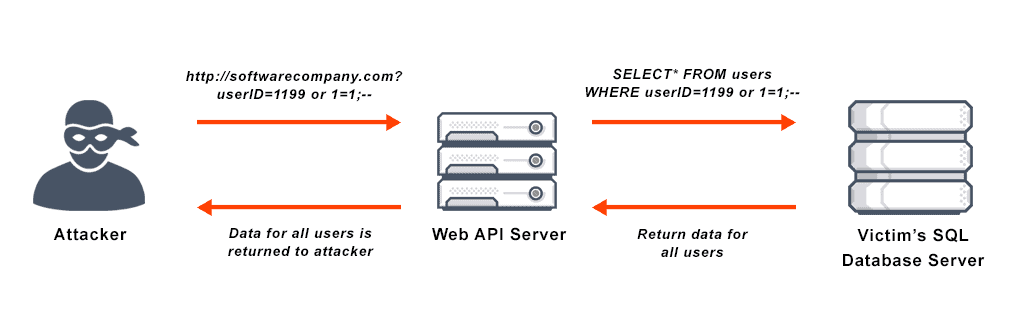
\includegraphics[height=0.2\textheight]{sql-injection_schema.png}
    \caption[Visualisatie van een sql-injection aanval]{Visualistie van een sql-injection aanval}
\end{figure}
\subsubsection{\IfLanguageName{dutch}{SQL-injectie}{SQL-injection}}
\label{sec:SQL-injectie}

SQL-injectie is een veelvoorkomende cyberbeveiligingsdreiging waarbij aanvallers schadelijke SQL-code injecteren in webapplicaties om databases te manipuleren. 
Dit omvat het stelen van gegevens, het wijzigen van records of zelfs het verwijderen van belangrijke informatie. Om dit te bestrijden, wordt inputvalidatie 
toegepast waarbij alle gebruikersinvoer wordt gecontroleerd en gefilterd om onveilige tekens en SQL-commando's uit te sluiten. Een andere effectieve methode 
is het gebruik van geparametriseerde queries, die de structuur van een SQL-query scheiden van de daadwerkelijke data, waardoor de kans op een succesvolle 
injectie wordt verkleind. Inbraakdetectiesystemen spelen ook een cruciale rol; dergelijke systemen monitoren netwerkverkeer op abnormale patronen die wijzen op 
een inbraakpoging, zoals ongewoon veel databaseverzoeken. Deze technieken samen verhogen de weerbaarheid van systemen tegen SQL-injectie aanvallen, elk 
aangepast aan de specifieke behoeften van de applicatie ~\autocite{Abdullayev2023}.

\subsubsection{\IfLanguageName{dutch}{Cross-Site Scripting (XSS)}{Cross-Site Scripting (XSS)}}
\label{sec:Cross-Site Scripting (XSS)}
\begin{figure}
    \centering
    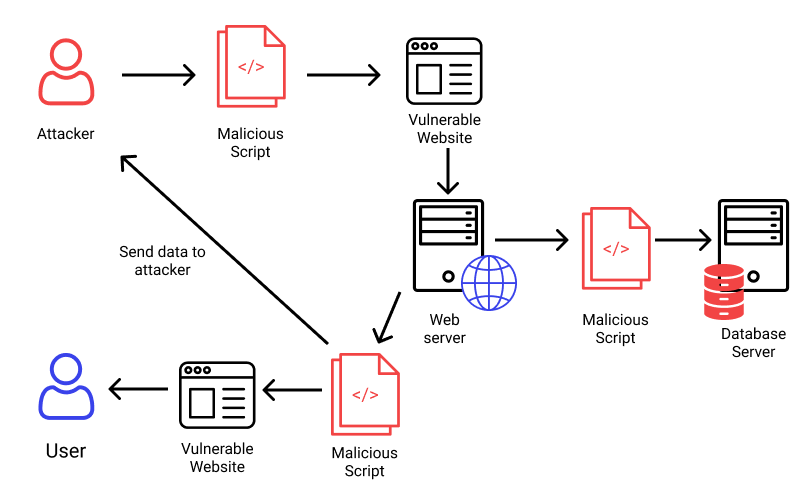
\includegraphics[height=0.3\textheight]{XSS_schema.png}
    \caption[Visualisatie van een XSS-aanval]{Visualisatie van een XSS-aanval}
\end{figure}

Cross-Site Scripting (XSS) is een type cyberaanval waarbij aanvallers kwaadaardige scripts op websites plaatsen, die vervolgens worden uitgevoerd door de 
browsers van gebruikers. Dit kan leiden tot gestolen cookies, waarbij aanvallers toegang krijgen tot opgeslagen sessiegegevens die authenticatie mogelijk 
maken. Sessiehijacking houdt in dat aanvallers de controle over de gebruikerssessie overnemen. Ook kan er manipulatie van de website-inhoud plaatsvinden, 
waardoor gebruikers misleidende informatie zien. Content Security Policies (CSP) zijn een cruciale verdedigingsmaatregel die bepaalt welke contentbronnen 
geldig zijn voor een website, waardoor het laden van ongeautoriseerde scripts wordt beperkt en zo wordt voorkomen dat XSS-aanvallen effectief kunnen zijn. 
Door het instellen van CSP's kunnen ontwikkelaars specifieke regels definiëren voor waar en hoe bronnen geladen mogen worden, wat een extra laag van beveiliging
biedt ~\autocite{Weamie2022}.

\subsubsection{\IfLanguageName{dutch}{Broken Access Control (BAC)}{Broken Access Control (BAC)}}
\label{sec:Broken Access Control (BAC)}

Broken Access Control (BAC) is een kwetsbaarheid in webapplicaties die ontstaat wanneer de toegangscontrolesystemen niet effectief de gebruikersactiviteiten beperken. 
Dit kan leiden tot situaties waarbij gebruikers acties kunnen uitvoeren waarvoor ze geen toestemming hebben. Dit omvat toegang tot gevoelige data, het wijzigen 
van gegevens zonder de juiste autorisatie, of het uitvoeren van functies die hun rechten overschrijden. De beveiliging tegen BAC vereist een zorgvuldige implementatie 
van toegangsbeleid dat zowel authenticatie als autorisatie controles omvat, waarbij moet worden gezorgd dat deze controles consistent en robuust worden toegepast over 
alle onderdelen van de applicatie \autocite{Anas2024}.

\subsubsection{\IfLanguageName{dutch}{Brute force aanvallen}{brute force attacks}}
\label{sec:brute force aanvallen}
Een brute force-aanval is een techniek waarbij aanvallers systematisch alle mogelijke combinaties van wachtwoorden of sleutels uitproberen om toegang te krijgen tot een 
systeem of account. Deze aanpak kan effectief zijn bij het kraken van zwakke wachtwoorden, vooral als er geen maatregelen zoals accountvergrendeling na meerdere mislukte 
pogingen zijn toegepast. Mensen voeren deze aanvallen uit met verschillende motieven, waaronder het stelen van persoonlijke of financiële informatie, het uitvoeren van 
frauduleuze transacties, of het saboteren van systemen. Dit benadrukt het belang van sterke wachtwoordbeleid en beveiligingsmaatregelen om dergelijke aanvallen te weerstaan
~\autocite{Djukanovic2020}.

\subsubsection{\IfLanguageName{dutch}{Cross-Site Request Forgery (CSRF)}{Cross-Site Request Forgery (CSRF)}}
\label{sec:brute force aanvallen}
Cross-Site Request Forgery (CSRF) is een type aanval waarbij een kwaadaardige website ongeautoriseerde acties uitvoert namens een gebruiker die bij een andere website is 
ingelogd. Deze acties kunnen variëren van het wijzigen van wachtwoorden tot het maken van financiële transacties. CSRF-aanvallen maken misbruik van de manier waarop 
webbrowsers automatisch inloggegevens, zoals cookies\footnote{Cookies zijn "minibestanden" en kunnen worden geplaatst op uw apparaat dat is verbonden met het internet, 
zoals een computer, telefoon, tablet of smart TV. Cookies kunnen worden gebruikt om informatie te verzamelen of op te slaan over hoe u zich gedraagt op een website 
en/of op uw apparaat}, meesturen bij het maken van verzoeken naar een webserver. Om deze aanvallen tegen te gaan, gebruiken ontwikkelaars 
vaak anti-CSRF tokens, die moeten worden meegezonden met elk verzoek dat een side-effect heeft. Zonder het juiste token wordt het verzoek geweigerd, wat helpt om de 
gebruiker te beschermen tegen ongewilde acties ~\autocite{B.I.2024}.

\begin{figure}
    \centering
    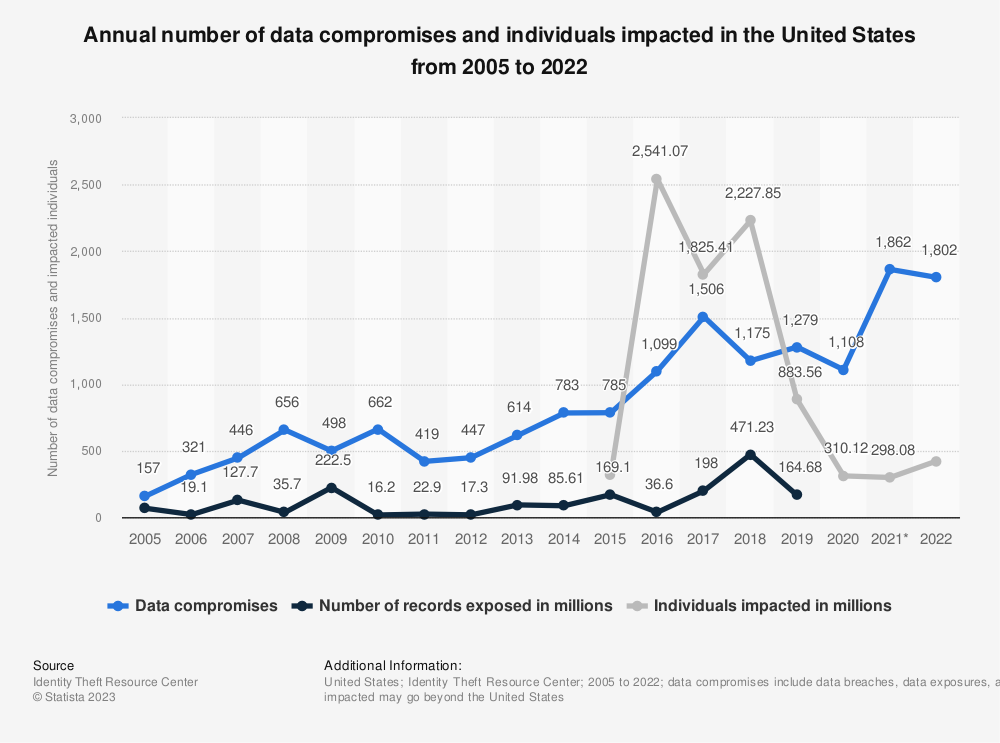
\includegraphics[height=0.3\textheight]{data-breaches-statistics-us.png}
    \caption[Aantal data breaches in de US ]{Aantal data breaches in de US }
    \label{fig:data-breaches}
\end{figure}

\subsection{\IfLanguageName{dutch}{Security mechanismen in websites en webapplicaties}{Security mechanisms in websites and web applications}}
\label{sec:Security mechanismen in Webomgevingen}

In dit hoofdstuk worden de security mechanismen van de drie verschillende webomgevingen onderzocht. Elk platform heeft zijn eigen beveiligingsmaatregelen die bijdragen 
aan de algehele veiligheid van webapplicaties.

WordPress, een veelgebruikt content management systeem, bevat enkele ingebouwde beveiligingsfuncties zoals gebruikersrollen, beveiligde 
wachtwoorden en bestandsrechten. Hoewel deze maatregelen helpen bij het beschermen van een website, vooral tegen basisaanvallen, zijn ze 
mogelijk niet afdoende tegen geavanceerde bedreigingen zoals SQL-injecties en cross-site scripting (XSS). Het gebruik van aanvullende 
beveiligingsmaatregelen, zoals beveiligingsplugins, wordt daarom aanbevolen, vooral voor websites die gevoelige informatie verwerken 
of een hoog risico lopen op aanvallen~\autocite{Trunde2015}

Wordfence, een vooraanstaande beveiligingsplugin voor WordPress, biedt een uitgebreide suite van beveiligingsfuncties, waaronder een 
firewall, malware scanner en DDoS bescherming. Deze plugin is speciaal ontworpen om WordPress-websites te beschermen tegen bekende 
bedreigingen en om verdachte activiteiten in realtime te monitoren. De effectiviteit van Wordfence in het verdedigen van WordPress-sites 
tegen een breed scala aan aanvallen is erkend en heeft bijgedragen aan zijn reputatie als een betrouwbare beveiligingsoplossing voor 
WordPress-gebruikers~\autocite{277144}.

Laravel, een krachtig PHP-framework, geniet bekendheid vanwege zijn geavanceerde beveiligingsfuncties en solide architectuur. Het 
framework biedt ingebouwde bescherming tegen veelvoorkomende beveiligingskwetsbaarheden, zoals CSRF-aanvallen en SQL-injecties, wat 
bijdraagt aan de veiligheid van webapplicaties die op Laravel zijn gebouwd. Bovendien biedt Laravel's uitgebreide authenticatie- en 
autorisatiesysteem ontwikkelaars een gestandaardiseerde en veilige methode om gebruikers te beheren en toegangscontroles toe te passen. 
Deze functies maken Laravel een populaire keuze voor ontwikkelaars die streven naar veilige en betrouwbare webapplicaties
~\autocite{Adamu2020}.

De piek in datalekken in 2016 die je kan terugvinden op figuur \ref{fig:data-breaches} is grotendeels te danken aan enkele grootschalige datalekken, zoals het Yahoo-datalek waarbij 
drie miljard gebruikersaccounts werden getroffen. De daling in 2018 daarentegen, kan worden verklaard door verbeterde beveiligingsmaatregelen 
en de invoering van strengere gegevensbeschermingswetten zoals de AVG in Europa ~\autocite{Petrosyan2024}. Deze gebeurtenissen benadrukken het belang van 
robuuste security mechanismen. Door te investeren in geavanceerde beveiligingstools en gebruik te maken van veilige 
frameworks zoals Laravel, kunnen organisaties hun weerbaarheid tegen cyberaanvallen aanzienlijk verhogen en de veiligheid van hun 
gegevens waarborgen ~\autocite{Petrosyan2024}.

Het toevoegen van beveiligingsplugins zoals Wordfence aan WordPress kan de beveiliging aanzienlijk verbeteren, terwijl Laravel van nature een 
sterke beveiligingslaag biedt. Het kiezen van het juiste platform hangt daarom af van de specifieke behoeften van het project en de nadruk op beveiliging.
\section{\IfLanguageName{dutch}{Pentesting tools}{Pentesting tools}}
\label{sec:Pentesting tools}
Bij het kiezen van de juiste pentesting tools voor webomgevingen moet worden overwogen welke functionaliteiten 
elke tool biedt. Dit is van cruciaal belang, gezien de vele verschillende soorten webapplicaties en de bijbehorende veiligheidsrisico's.

Een van de eerste aspecten waarop moet worden gelet, is of de tool geschikt is voor de specifieke behoeften. Sommige tools 
zijn specifiek ontworpen voor het testen van websites, terwijl andere meer geschikt zijn voor het evalueren van volledige 
netwerken. Het is essentieel om een tool te selecteren die aansluit bij de specifieke vereisten van de situatie. Het 
is dan ook logisch om voor verschillende taken verschillende tools te gebruiken~\autocite{Deepikakongara2023}.
Zoals aangehaald in het eerste hoofdstuk, is het belangrijk om rekening te houden met de grootte van het netwerk, 
het soort infrastructuur en het type kwetsbaarheden dat wordt getest.

Gebruiksgemak in de keuze van de juiste tool is eveneens van belang, vooral wanneer niet alle teamleden experts zijn. Een tool zoals OWASP ZAP, 
die gebruiksvriendelijk is, kan aanzienlijk veel tijd besparen en de toegankelijkheid voor alle teamleden vergroten.
Daarnaast biedt een analyse, toegankelijk via Google Books, een volledige vergelijking tussen enkele van de meest gekende pentesting tools op de markt, 
zoals Nmap, Burp Suite, en OWASP ZAP. Deze bron is bijzonder waardevol voor professionals binnen de cybersecurity wereld, omdat het inzicht geeft in de sterke en zwakke 
punten van elk van deze tools. Door deze tools te vergelijken, kunnen teams betere beslissingen nemen over welke het meest geschikt zijn 
voor hun specifieke beveiligingsbehoeften ~\autocite{Velu2022}.

Regelmatige updates zijn van groot belang om ervoor te zorgen dat de tool in staat blijft om nieuwe kwetsbaarheden te 
identificeren. Het is belangrijk om niet achter te blijven en verouderde bedreigingen te testen terwijl kwaadwillende 
partijen al nieuwe methoden hebben ontwikkeld.

Een bijzonder effectieve tool binnen het domein van pentesting is Metasploit. Metasploit is een uitgebreid platform voor het uitvoeren van 
penetratietesten en wordt algemeen erkend door zijn kracht. De tool maakt gebruik van een uitgebreide database met exploits en 
payloads, waardoor testers in staat zijn om verschillende aanvalstechnieken te simuleren en te testen. Bovendien biedt Metasploit ondersteuning 
voor zowel automatische als handmatige tests, wat de flexibiliteit vergroot en het geschikt maakt voor zowel beginners als gevorderde gebruikers. 
De voortdurende updates en de mogelijkheid om modules te integreren maken Metasploit tot een handige tool voor elke 
beveiligingsprofessional ~\autocite{Rani2019}. 

Natuurlijk spelen budgettaire overwegingen ook een rol, aangezien pentest-tools variëren van gratis tot zeer prijzig. Het 
is van belang om een tool te vinden die binnen het budget past maar tegelijkertijd voldoet aan de vereiste functionaliteiten
om de gewenste veiligheid te waarborgen.

Ten slotte moet de tool voldoende diepgaand zijn om zowel oppervlakkige als meer verborgen problemen aan te pakken. 
Een goede tool kan helpen bij het identificeren en verhelpen, van kleine fouten tot ernstige beveiligingslekken
~\autocite{Maji2022}.

Door deze bovenstaande aspecten af te wegen, kunnen de juiste tools worden geselecteerd voor pentestingwerkzaamheden. 
Dit kan veel bijdragen aan het verbeteren van de veiligheid van webomgevingen en het uitvoeren van effectievere beveiligingstests.

\section{\IfLanguageName{dutch}{Wat weten we uit de literatuur}{What is known from the literature}}
\label{sec:wat-weten-we-uit-de-literatuur}
Beveiliging van webapplicaties is een noodzakelijk onderwerp geworden. Recente onderzoeken en literatuur leveren 
inzichten in verschillende aspecten van dit vakgebied, waaronder de effectiviteit van penetratietests, het belang van beveiligingsplugins voor WordPress en de verschillen 
in beveiligingsmaatregelen tussen webapplicatieframeworks zoals Laravel. Een overzicht van wat reeds gekend is op dit gebied, ondersteund door een aantal 
bronnen, toont de huidige kennis en praktijken aan.

Cybersecurity-instrumenten spelen een cruciale rol, bijvoorbeeld bij penetratietests binnen webomgevingen. Een weloverwogen keuze bij het
selecteren van effectieve tools van belang, zoals in het vorig hoofdstuk aangehaald, om kwetsbaarheden in webapplicaties te identificeren en aan te pakken. 
Deze selectie vereist niet alleen technische kennis, maar ook strategisch inzicht in hoe verschillende tools verschillende 
soorten beveiligingslekken kunnen identificeren.
Een doordachte aanpak bij het kiezen van penetratietesttools versterkt niet alleen de beveiligingshouding 
van organisaties, maar verbetert ook hun vermogen om zich aan te passen aan nieuwe bedreigingen. 

Het consequent toepassen van deze tools helpt niet alleen bij het identificeren van onmiddellijke dreigingen, maar 
biedt ook inzichten in potentiële toekomstige kwetsbaarheden ~\autocite{Albahar2022}.
Daarnaast draagt een effectieve beveiligingsstrategie bij aan het opbouwen van vertrouwen bij klanten en gebruikers, die er 
zeker van kunnen zijn dat hun gegevens veilig worden beheerd. 

In het licht van toenemende regelgeving rond gegevensbescherming 
is het van groot belang dat organisaties niet alleen voldoen aan de industrienormen, maar deze zelfs overtreffen.
Dus, terwijl de technologie blijft evolueren, is het van cruciaal belang dat beveiligingsteams hun tools voortdurend 
beoordelen en bijwerken, zodat ze voorbereid zijn op zowel de huidige als toekomstige cyberuitdagingen. Dit continue 
proces van beoordeling en verbetering is noodzakelijk voor het bewaren van een sterke verdediging tegen een breed scala 
aan internetbedreigingen.

Een belangrijk aspect van onderzoek draait om de impact van beveiligingsplugins op WordPress-websites. Deze plugins, zoals Wordfence en iThemes Security, worden 
erkend vanwege hun vermogen om een cruciale beveiligingslaag toe te voegen aan WordPress-sites. Ze zijn speciaal ontworpen om de vele bedreigingen af 
te weren, waardoor ze een belangerijk onderdeel vormen van de beveiligingsstrategie voor elke WordPress-omgeving~\autocite{Casola2020}.

Een rapport dat werd gepresenteerd, onderzoekt de drie belangrijkste beveiligingsrisico's geïdentificeerd door OWASP en verkent hoe penetratietesttools kunnen 
worden ingezet om deze bedreigingen bij websites op te sporen. Het voornoemde rapport bespreekt ook hoe 
penetratietesttools kunnen worden ingezet om deze bedreigingen bij websites op te sporen, wat cruciaal is voor organisaties die hun cyberweerbaarheid willen verbeteren
~\autocite{Sharma2023}.

Als het CMS-systeem WordPress vergelijkt word met het Laravel-framework, valt op dat dit laatste beveiligingsvoordelen biedt. Deze voordelen worden voornamelijk toegeschreven aan 
de robuuste architectuur van Laravel, die inherent meer beveiligingslagen biedt. Laravel maakt gebruik van moderne beveiligingspraktijken en heeft ingebouwde 
functies die helpen bij het beschermen tegen veelvoorkomende bedreigingen zoals SQL-injecties, cross-site scripting (XSS) en cross-site request forgery (CSRF)~\autocite{Lebedeva2023}. Deze focus 
op beveiliging maakt Laravel een aantrekkelijke keuze voor ontwikkelaars en bedrijven die de veiligheid van hun webapplicaties serieus nemen en zich bewust 
zijn van de toenemende dreigingen op het internet. De voordelen van Laravel op het gebied van beveiliging zijn dus een belangrijke overweging voor organisaties 
bij het selecteren van een framework voor hun projecten.

Samenvattend laten deze studies zien wat er bekend is over de beveiliging van webapplicaties.
Het is essentieel om inzicht te krijgen in de specifieke beveiligingsproblemen die elk webapplicatieframework met zich meebrengt. Door deze inzichten 
toe te passen kunnen organisaties hun beveiligingshouding versterken en beter beschermen tegen de voortdurende dreiging van cyberaanvallen.

\section{\IfLanguageName{dutch}{Wat weten we niet uit de literatuur?}{What is not known from the literature?}}
Hoewel de bestaande literatuur een waardevolle kijk biedt op het vlak van webapplicatiebeveiliging en de effectiviteit van penetratietesting, blijven er nog 
zaken die niet volledig worden beantwoord. Uit de analyse van twee specifieke bronnen, de conferentieproceedings van CyberCon en een publicatie in het 
Computer Science and Information Technology (CS and IT) tijdschrift, komen enkele van deze tekorten aan bod.

Het artikel op de CyberCon-conferentie bespreekt de cybersecurity van WordPress-platformen, specifiek door het gebruik van attack-defense trees. Deze methode helpt 
bij het analyseren en visualiseren van verschillende aanvals- en verdedigingsscenario's, wat fundamenteel is voor een diepgaand begrip van mogelijke bedreigingen en 
effectieve tegenmaatregelen. Dit is bijzonder relevant in het licht van de complexiteit van nieuwe cyberaanvallen die geavanceerde technologieën zoals AI en machine 
learning gebruiken. Een typisch voorbeeld hiervan zijn AI-gestuurde phishing-campagnes zoals chatbots. De chatbots maken zeer goede en overtuigende teksten, die niet als 
phishing-tekst herkenbaar zijn. Een ander voorbeeld zijn machine learning methodes die beveiligingspatronen herkennen en exploiteren. Deze nieuwe aanvalstechnieken
focussen op de pijnpunten binnen de cybersecurity zoals de menselijke factor en de complexiteit van beveiligingsmaatregelen. Menselijke fouten vormen een belangrijk 
deel van de zwakten van cyberbeveiliging. Het kan bijvoorbeeld enorm moeilijk zijn om de juiste systeemconfiguratie te beheren, ook als daarvoor grote IT-teams worden 
ingezet ~\autocite{Petrica2022}.

Daarnaast wijst een studie gepubliceerd in het CS and IT tijdschrift op het ontbreken van benchmarks en vergelijkende studies die de prestaties van verschillende 
beveiligingsplugins en frameworks onder bepaalde omstandigheden beoordelen. Dit gebrek aan vergelijkend onderzoek maakt het voor ontwikkelaars 
moeilijk om onderbouwde beslissingen te nemen bij de implementatie van beveiligingsmaatregelen binnen hun webapplicaties. De studie benadrukt de noodzaak voor 
het maken van benchmarks, die van belang zijn bij het vinden van de meest effectieve beveiligingsaanpakken tegen diverse cyberdreigingen ~\autocite{AbuDabaseh2018}.

Beide bronnen tonen het belang van voortdurend onderzoek naar en ontwikkeling van penetratietesting methodologieën, beveiligingsplugins en frameworks om te kunnen 
blijven voldoen aan de eisen van een voortdurend veranderende omgeving. Ze benadrukken dat, hoewel veel bekend is over de basisprincipes van webapplicatiebeveiliging, 
de details van het beschermen tegen de nieuwste en meest geavanceerde aanvalstechnieken nog ontdekt moeten worden. Dit duidt op een enorme behoefte aan 
specifiek onderzoek en praktijkexperimenten om de effectiviteit van bestaande en nieuwe beveiligingsmethoden te verbeteren.

\section{\IfLanguageName{dutch}{Relevantie van het onderzoek}{Relevance of the study}}
\subsection{\IfLanguageName{dutch}{Theoretische relevantie}{Theoretical relevance}}
De analyse van penetratietesttools in specifieke webomgevingen speelt een cruciale rol in het versterken van webapplicatiebeveiliging. Door deze tools 
te evalueren, wordt inzicht verkregen in hoe ze kwetsbaarheden identificeren en aanpakken, wat essentieel is voor het opstellen van robuuste beveiligingsprotocollen. 
Een goed begrip ervan helpt bij het optimaliseren van beveiligingsstrategieën en het anticiperen op mogelijke aanvallen, waardoor organisaties beter voorbereid zijn op het 
afweren van cyberdreigingen. Dit draagt dan op zijn beurt bij aan een veiligere digitale omgeving, waarbij de focus ligt op preventie en effectieve respons
~\autocite{Jarupunphol2023}.

De verkregen inzichten uit de analyse van verschillende penetratietesttools binnen een specifieke webomgeving zijn zeer waardevol. Ze bieden gedetailleerde informatie 
over de methoden die deze tools gebruiken om kwetsbaarheden te identificeren en te analyseren. Dit draagt bij aan een breder begrip van de dynamiek van pentesting, waarmee 
wordt bedoeld het begrijpen van de verschillende tactieken, technieken en procedures die pentesters gebruiken om beveiligingslekken te vinden en te verhelpen. Het 
begrijpen van deze processen is van belang voor professionals in de cybersecurity en webapplicatieontwikkeling, wat hen helpt bij het implementeren van effectievere 
beveiligingsstrategieën.

De integratie van beveiligingstechnieken en theoretische concepten, zoals vermeld in het artikel gepubliceerd in IJITEE, is cruciaal. Deze spelen een belangrijke rol 
in het bijeenbrengen van bestaande theoretische modellen en de praktische uitdagingen van webbeveiliging. Dit onderzoek maakt gebruik van de nieuwste inzichten in cybersecurity 
om bestaande theoretische kaders te evalueren. En draagt bovendien bij aan de ontwikkeling van vernieuwde theorieën die de complexe problemen van hedendaagse 
cyberdreigingen beter weergeven. Door hedendaagse beveiligingsconcepten te koppelen aan de analyse van penetratietesttools binnen specifieke webomgevingen, 
stimuleert het onderzoek de evolutie van theoretische benaderingen in cybersecurity. Tegelijkertijd levert het belangerijke inzichten voor het implementeren van beveiligingsmaatregelen
die overeenkomen met de realiteit van de huidige digitale computercriminaliteit.
Dit proces draagt bij aan het verfijnen en versterken van webbeveiligingspraktijken, gericht op het voldoende beschermen tegen en reageren op moderne 
cyberdreigingen~\autocite{Nagendran2019}.

\subsection{\IfLanguageName{dutch}{Maatschappelijke relevantie}{Social relevance}}
Door inzichten uit geavanceerde onderzoeken te integreren, vergroot dit onderzoek de maatschappelijke relevantie van webapplicatiebeveiliging. Hiervoor wordt er verwezen naar 
twee cruciale bronnen: een studie van ArXiv en een onderzoek gepubliceerd in het eJournal of ICT van Akademi Telkom Jakarta. Beide bronnen bieden een uitgebreid overzicht 
van de huidige uitdagingen op het gebied van cybersecurity en de implementatie van geavanceerde beveiligingsmaatregelen en bieden de nodige perspectieven die het 
belang van dit onderzoek aan het licht brengen.

Het ArXiv-document presenteert een gedetailleerde analyse van nieuwe cybersecuritydreigingen, waaronder aanvallen die gebruikmaken van geavanceerde technologieën zoals 
kunstmatige intelligentie (AI) en machine learning. Een voorbeeld hiervan, eerder aangehaald in deze studie, zijn de geautomatiseerde phishing-aanvallen door middel van chatbots waarbij AI ingezet om 
gepersonaliseerde en overtuigende phishingberichten te creëren die specifiek zijn afgestemd op het gedrag en de voorkeuren van gebruikers. Deze technologieën worden ingezet om 
aanvalspatronen te optimaliseren en detectiesystemen te omzeilen, waardoor de dreigingen steeds complexer worden. Dit benadrukt de noodzaak voor webapplicaties om hun 
beveiligingsmaatregelen voortdurend te updaten en te versterken om effectieve bescherming tegen deze evoluerende dreigingen te bieden ~\autocite{Deng2023}.

Tegelijkertijd gaat de studie gepubliceerd in het eJournal of ICT van Akademi Telkom Jakarta in op specifieke beveiligingsmaatregelen en hun effectiviteit in 
het beschermen van webapplicaties tegen geavanceerde cyberaanvallen. Dit onderzoek draagt bij aan de maatschappelijke impact door een praktische kijk te 
bieden in de implementatie van deze beveiligingsmaatregelen en toont hun doeltreffendheid in real-world scenario's aan. Door succesvolle strategieën voor het 
verdedigen tegen cyberaanvallen te presenteren, dient deze studie als een waardevolle bron voor ontwikkelaars, beveiligingsprofessionals en organisaties
die ernaar streven de beveiligingshouding van webapplicaties te versterken ~\autocite{OlivianaZabka2023}.

De maatschappelijke relevantie van dit onderzoek is veelzijdig. Het draagt direct bij tot het verbeteren van de digitale veiligheid en privacy van personen 
en organisaties die afhankelijk zijn van webapplicaties voor verschillende aspecten van hun dagelijks leven. Bij het overwegen van de huidige situatie waarin 
digitale dreigingen ernstige economische en sociale gevolgen kunnen hebben, bieden de inzichten uit de ArXiv- en eJournal of ICT-studies waardevolle informatie. Deze strategieën 
verminderen niet alleen het risico op datalekken en cyberaanvallen, maar bouwen ook vertrouwen op in digitale platforms onder gebruikers.

Samengevat, maatschappelijk levert dit onderzoek een fundamentele bijdrage aan het verbeteren van de digitale veiligheid en het vertrouwen in webapplicaties, die essentieel 
zijn in het dagelijks leven van zowel individuen als organisaties. Door te concentreren op de meest actuele cybersecurity-uitdagingen en oplossingen, 
helpt het bij het maken van nieuwe regels en wetten, en roept op tot strengere beveiligingsstandaarden. Het biedt niet alleen strategieën om het risico 
op datalekken en cyberaanvallen te verminderen, maar versterkt ook het vertrouwen in digitale platformen. Zo draagt het onderzoek bij aan een veiligere 
digitale omgeving in een tijd waarin de digitale dreigingen significante economische en sociale impact kunnen hebben.

%Dit hoofdstuk bevat je literatuurstudie. De inhoud gaat verder op de inleiding, maar zal het onderwerp van de bachelorproef *diepgaand* uitspitten. De bedoeling is dat de lezer na lezing van dit hoofdstuk helemaal op de hoogte is van de huidige stand van zaken (state-of-the-art) in het onderzoeksdomein. Iemand die niet vertrouwd is met het onderwerp, weet nu voldoende om de rest van het verhaal te kunnen volgen, zonder dat die er nog andere informatie moet over opzoeken \autocite{Pollefliet2011}.

%Je verwijst bij elke bewering die je doet, vakterm die je introduceert, enz.\ naar je bronnen. In \LaTeX{} kan dat met het commando \texttt{$\backslash${textcite\{\}}} of \texttt{$\backslash${autocite\{\}}}. Als argument van het commando geef je de ``sleutel'' van een ``record'' in een bibliografische databank in het Bib\LaTeX{}-formaat (een tekstbestand). Als je expliciet naar de auteur verwijst in de zin (narratieve referentie), gebruik je \texttt{$\backslash${}textcite\{\}}. Soms is de auteursnaam niet expliciet een onderdeel van de zin, dan gebruik je \texttt{$\backslash${}autocite\{\}} (referentie tussen haakjes). Dit gebruik je bv.~bij een citaat, of om in het bijschrift van een overgenomen afbeelding, broncode, tabel, enz. te verwijzen naar de bron. In de volgende paragraaf een voorbeeld van elk.

%\textcite{Knuth1998} schreef een van de standaardwerken over sorteer- en zoekalgoritmen. Experten zijn het erover eens dat cloud computing een interessante opportuniteit vormen, zowel voor gebruikers als voor dienstverleners op vlak van informatietechnologie~\autocite{Creeger2009}.

%Let er ook op: het \texttt{cite}-commando voor de punt, dus binnen de zin. Je verwijst meteen naar een bron in de eerste zin die erop gebaseerd is, dus niet pas op het einde van een paragraaf.

%\lipsum[7-20]

%%=============================================================================
%% Methodologie
%%=============================================================================

\chapter{\IfLanguageName{dutch}{Methodologie}{Methodology}}%
\label{ch:methodologie}

%% TODO: In dit hoofstuk geef je een korte toelichting over hoe je te werk bent
%% gegaan. Verdeel je onderzoek in grote fasen, en licht in elke fase toe wat
%% de doelstelling was, welke deliverables daar uit gekomen zijn, en welke
%% onderzoeksmethoden je daarbij toegepast hebt. Verantwoord waarom je
%% op deze manier te werk gegaan bent.
%% 
%% Voorbeelden van zulke fasen zijn: literatuurstudie, opstellen van een
%% requirements-analyse, opstellen long-list (bij vergelijkende studie),
%% selectie van geschikte tools (bij vergelijkende studie, "short-list"),
%% opzetten testopstelling/PoC, uitvoeren testen en verzamelen
%% van resultaten, analyse van resultaten, ...
%%
%% !!!!! LET OP !!!!!
%%
%% Het is uitdrukkelijk NIET de bedoeling dat je het grootste deel van de corpus
%% van je bachelorproef in dit hoofstuk verwerkt! Dit hoofdstuk is eerder een
%% kort overzicht van je plan van aanpak.
%%
%% Maak voor elke fase (behalve het literatuuronderzoek) een NIEUW HOOFDSTUK aan
%% en geef het een gepaste titel.

In de initiële fase van dit onderzoek, de literatuurstudie, werd de focus gelegd op het verzamelen van bestaande kennis 
en onderzoek op het gebied van webapplicatiebeveiliging, pentesting-tools en frameworks, met een specifieke nadruk op 
WordPress en Laravel. Deze fase was van cruciaal 
belang om een stevige basis te leggen voor mijn onderzoek en om de context en achtergrond van het onderwerp volledig te 
begrijpen.

Om dit te bereiken, heb ik verschillende bronnen geraadpleegd, waaronder wetenschappelijke artikelen, boeken  
en rapporten van bekende instellingen en experts op het gebied van cybersecurity. 
Ik heb zoekopdrachten uitgevoerd in diverse academische databases, zoals PubMed, research gate en 
Google Scholar, om relevante literatuur te op nemen in mijn studie. Deze literatuur heb ik grondig geanalyseerd en 
samengevat, waarbij ik de nadruk heb gelegd op recente ontwikkelingen, trends en mogelijke tekortkomingen in de bestaande markt.
Ook werd in dit deel het globale aspect van cybersecutiy onder de loep genomen waardoor er een zeer duidelijk begrip 
is van de noden en hoe hierop een antwoord wordt gegeven.

\section{\IfLanguageName{dutch}{Requirements Analyse}{Requirements analysis}}
De requirements analyse vormt een cruciaal luik en beschrijft de methoden en technieken die worden toegepast 
voor het uitvoeren van penetratietests. In deze studie worden deze toegepast op drie 
verschillende webomgevingen met name een WordPress CMS-framework zonder beveiligingsplugins, een WordPress-framework met 
beveiligingsplugins, en een Laravel-applicatie. Het doel van deze tests is om kwetsbaarheden te identificeren, te 
analyseren en de effectiviteit van de beveiligingsmaatregelen in de verschillende omgevingen te vergelijken.
Deze 3 webomgevingen worden geselecteerd op basis van hun populariteit en relevantie voor kleine tot middelgrote bedrijven 
zoals webdevelopment firma Sinergio, die de partner en co-promotor is in dit onderzoek.

Voorafgaand aan de uitvoering van de penetratietests wordt toestemming verkregen van de beheerders van deze 
webomgevingen. Er wordt een identieke testomgeving opgezet om de impact op de live systemen te minimaliseren. 
Alle tests worden uitgevoerd in overeenstemming met de ethische richtlijnen voor cybersecurity onderzoek, 
waarbij de integriteit van de geteste systemen voorop staat.

Voor dit onderzoek worden drie verschillende penetratietesttools ingezet, elk geselecteerd vanwege hun 
specifieke sterktes in het identificeren en exploiteren van bepaalde soorten kwetsbaarheden:

\begin{itemize}
    \item Tool 1 wordt gebruikt voor de eerste webomgeving, een WordPress-applicatie zonder 
    beveiligingsplugins. Deze tool moet bijzonder geschikt voor het detecteren van webgebaseerde kwetsbaarheden 
    zoals SQL-injecties en cross-site scripting (XSS), waardoor het een uitstekende keuze is voor 
    een basis WordPress-installatie.
    \item Tool 2 wordt ingezet voor de tweede webomgeving, een WordPress-applicatie met beveiligingsplugins. 
    Deze tool excelleert in het omzeilen van beveiligingsmaatregelen en het uitvoeren van geautomatiseerde 
    aanvallen, waaronder brute force aanvallen. Dit maakt het bijzonder geschikt voor het grondig 
    testen van beveiligde WordPress-installaties.
    \item Tool 3 wordt gekozen voor de derde webomgeving, een Laravel-applicatie. Deze tool staat 
    bekend om zijn vermogen om specifieke framework-kwetsbaarheden te exploiteren en biedt functionaliteiten 
    die cruciaal zijn voor het testen van complexe applicaties zoals die gebouwd met Laravel.
\end{itemize}

Alle resultaten van de tests worden verzameld en gedocumenteerd. De data wordt geanalyseerd 
om de ernst en de impact van elke gevonden kwetsbaarheid te bepalen. Deze analyse helpt niet alleen bij 
het identificeren van de zwakke punten binnen elke webomgeving, maar ook bij het vergelijken van de 
veiligheid tussen de verschillende systemen. Ook wordt er gekeken naar de gebruiksvriendelijkheide en 
effectiviteit van de testen door een brute force aanval te simuleren op de wordpress applicatie met beveiligingsplugins.

\section{\IfLanguageName{dutch}{Keuze van Penetratietesttools}{Selection of pentesttools}}
In het kader van dit onderzoek naar de beveiliging van de drie verschillende webomgevingen is de keuze van 
de juiste penetratietesttools cruciaal. Voor elk van deze omgevingen is een tool geselecteerd die het 
best past bij de specifieke kenmerken en beveiligingsuitdagingen. De geselecteerde tools zijn 
Metasploit, Burp Suite en OWASP ZAP, waarbij hierna wordt toegelicht wat hen bijzonder geschikt maken voor dit onderzoek.
\begin{figure}
    \centering
    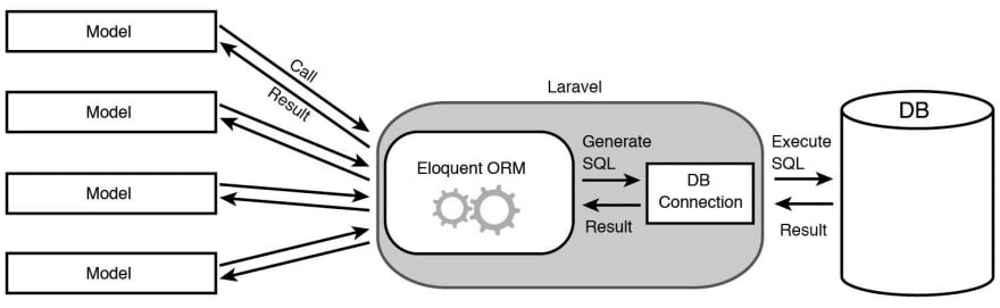
\includegraphics[height=0.2\textheight]{laravel_schema.png}
    \caption[Laravel ORM schema (Eloquent)]{Laravel ORM shema (Eloquent)}
\end{figure}
\subsection{\IfLanguageName{dutch}{Metasploit voor de Laravel-applicatie}{Metasploit for the Laravel application}}
Metasploit is een van de meest uitgebreide security frameworks voor het uitvoeren van penetratietests en 
staat bekend om zijn robuuste exploit-database en modulaire aanpak zoals ik heb vermeld in het hoofdstuk 
\nameref{sec:Webomgevingen} van de literatuurstudie. De Laravel-applicatie, bekend 
om zijn rijke set aan functionaliteiten en complexe architectuur, kan profiteren van Metasploit's 
vermogen om specifieke exploits te gebruiken die zijn afgestemd op gedetecteerde kwetsbaarheden. 
De tool biedt geautomatiseerde exploitatie technieken die essentieel zijn voor het identificeren 
van beveiligingsrisico's in een geavanceerd framework zoals Laravel. Bovendien ondersteunt 
Metasploit de ontwikkeling van aangepaste exploits, wat van grote waarde kan zijn bij 
het testen van functies binnen de te testen Laravel-applicatie.

\subsection{\IfLanguageName{dutch}{Burp Suite voor de wordpress applicatie met beveiligings plugins}{Burp Suite for the wordpress application with security plugins}}
Burp Suite is een geïntegreerd platform voor het testen van de beveiliging van webapplicaties en is 
bijzonder effectief voor het analyseren van HTTP-verkeer en het uitvoeren van geavanceerde web 
aanvallen. Zoals besproken in het hoofdstuk \nameref{sec:Webomgevingen} binnen de literatuurstudie 
biedt Burp Suite uitgebreide functionaliteiten die van belang zijn voor een grondige beveiligingsanalyse 
van webomgevingen. Voor een WordPress-installatie met beveiligingsplugins biedt Burp Suite daarom de noodzakelijke 
diepgang om de effectiviteit van de plugins te evalueren. Door zijn vermogen om verzoeken te 
onderscheppen, te manipuleren en opnieuw te versturen, kunnen testers de robuustheid van 
beveiligingsmaatregelen zoals firewalls en inbraakdetectiesystemen die door plugins worden 
geïmplementeerd, nauwkeurig beoordelen. Burp Suite's scanner, die vervat zit in de enterprise edition kan automatisch een breed scala 
aan kwetsbaarheden identificeren, wat tijd bespaart tijdens de testfase en zorgt voor een 
grondige evaluatie van de beveiligingsstatus.

\subsection{\IfLanguageName{dutch}{OWASP ZAP voor de wordpress applicatie zonder beveiligings plugins}{OWASP ZAP for the wordpress application without security plugins}}
OWASP ZAP (Zed Attack Proxy) is een open-source tool voor het automatisch detecteren van beveiligingsfouten 
in webapplicaties tijdens het ontwikkelings- en testproces. Gezien zijn goede reputatie en uitgebreide 
ondersteuning door de OWASP-community is ZAP bijzonder geschikt voor het testen van een 
WordPress-site zonder aanvullende beveiligingsmaatregelen. ZAP's geïntegreerde scanner en 
intercepting proxy maken het eenvoudig om kwetsbaarheden zoals XSS en SQL-injectie aan te 
tonen, die voorkomen in basisconfiguraties van WordPress. Daarnaast biedt ZAP dynamische 
analyse van de applicatie in real-time, wat helpt bij het direct identificeren van beveiligingsproblemen.


\section{\IfLanguageName{dutch}{Proof of Concept: Gebruiksvriendelijkheid en Effectiviteit van Pentesting Tools voor Webapplicaties}{Proof of Concept: Usability and Effectiveness of Pentesting Tools for Web Applications}}

In de proof of concept testen we de drie verschillende webomgevingen met de vernoemde pentesting tools om hun bruikbaarheid en effectiviteit te evalueren. 
Deze benadering is gericht op het vergelijken van de uitkomsten van pentests in elke omgeving, waardoor kan vastgesteld worden hoe de 
beveiligingsuitdagingen en kwetsbaarheden verschillen.

\subsubsection{\IfLanguageName{dutch}{Omgevingsdiversiteit}{Environmental diversity}}
De aanpak in deze proof of concept is gebaseerd op een realistische benadering, waarbij de drie pentesting tools worden gebruikt die zijn afgestemd 
op de unieke kenmerken van elke omgeving. Het team van Sinergio begrijpt dat geen twee webomgevingen dezelfde zijn en daarom is het belangrijk om een breed scala 
aan tools in te zetten om alle mogelijke kwetsbaarheden en beveiligingsrisico's aan het licht te brengen.

Door deze diversiteit aan tools kan het team niet alleen de specifieke omgeving testen met de best passende tool, maar ook de algehele robuustheid en 
weerbaarheid van de systemen maximaliseren. Elke tool heeft zijn eigen sterke punten en specialiteiten, waardoor een uitgebreide evaluatie mogelijk 
is die verder gaat dan alleen de oppervlakte.

Door te variëren in de gebruikte tools, kan het team verschillende aanvalsscenario's simuleren en de reactie van de systemen daarop beoordelen. Dit 
stelt hen in staat om een diepgaand inzicht te krijgen in de beveiligingsstatus van elke omgeving en biedt waardevolle informatie voor het verbeteren 
van de algehele beveiliging.

\subsubsection{\IfLanguageName{dutch}{Focus van pentesttools}{Focus of the pentesttools}}
De evaluatie van de wordpress beveiligingsplugin wordt geëvalueerd met Burp Suite om op die manier de efficiëntie ervan te testen. De focus ligt op het evalueren van de weerstand 
tegen veelvoorkomende webaanvallen, zoals brute force-aanvallen en SQL-injectie. Ze analyseren hoe de plugin potentiële dreigingen behandelt met 
behulp van Burp Suite en identificeren eventuele tekortkomingen in de bescherming

OWASP ZAP helpt bij het blootleggen van kwetsbaarheden die een website zonder beveiligingsmaatregelen zou kunnen hebben. De nadruk ligt op het 
ontdekken van eenvoudig te exploiteren kwetsbaarheden en het trainen van aan nieuwe gebruikers om deze kwetsbaarheden te begrijpen en 
te leren hoe ze tegen te gaan.

Met Metasploit wordt gefocust op geavanceerdere beveiligingsaspecten, zoals routebescherming en authenticatiemechanismen.
In Laravel is het bijvoorbeeld mogelijk om het aantal mislukte inlogpogingen in te stellen voordat een gebruiker tijdelijk wordt geblokkeerd. Dit wordt vaak gedaan 
als een beveiligingsmaatregel om brute force-aanvallen te voorkomen. Je kunt het aantal inlogpogingen aanpassen door een eigenschap genaamd 
'maxAttempts' in te stellen in de configuratie van het authenticatiesysteem van Laravel. Deze tests zullen 
bijdragen aan het inzicht in de robuustheid van de beveiliging en helpen bij het identificeren van potentieel over het hoofd geziene kwetsbaarheden.

\section{\IfLanguageName{dutch}{Hoe pentesten}{How to pentest}}
Dit hoofdstuk beschrijft de methodologie die wordt gehanteerd voor het uitvoeren van penetratietesten op webapplicaties met behulp van Metasploit, 
Burp Suite Community Edition en OWASP ZAP. De focus ligt hierbij op twee specifieke aanvalstechnieken: brute force-aanvallen en SQL-injecties. 
Het gebruik van deze tools en technieken heeft tot doel inzicht te verkrijgen in de kwetsbaarheden van webapplicaties en de effectiviteit van 
verschillende beveiligingsmaatregelen.

\subsection{\IfLanguageName{dutch}{Voorbereiding van de testomgeving}{Voorbereiding van de testomgeving}}
Voor de uitvoering van de penetratietesten werd een gecontroleerde omgeving opgezet door Sinergio. Deze omgeving omvat een webserver waarop kwetsbare 
applicaties draaien, specifiek ontworpen om te dienen als testdoelen voor beveiligingsanalyses. Hiervoor is de server security via de firewall ook uitgezet zodat 
het IP nooit geblacklist zou worden wanneer een brute-force aanval wordt gesimuleerd. De gebruikte testapplicaties zijn gebaseerd 
op WordPress en Laravel, aangezien deze veelvoorkomende platforms representatief zijn voor echte wereldscenario's.

\subsection{\IfLanguageName{dutch}{Werkwijze metasploit}{Working method metasploit}}
Metasploit kan geïnstalleerd worden op een Windows-systeem. De installatie omvat de nieuwste versie van Metasploit Framework, samen met de 
benodigde updates en dependencies.

\subsubsection{\IfLanguageName{dutch}{Brute-force aanval}{Brute-force attack}}
Om een brute force-aanval uit te voeren met Metasploit op een webapplicatie, wordt gebruikgemaakt van de auxiliary\slash scanner\slash http\slash brute\_dirs
module. Deze module probeert verschillende URL-paden op de webserver te vinden door middel van brute force.
Het te volgen parcours gaat als volgt:
\begin{enumerate}
    \item Start Metasploit en laad de brute\_dirs module
    \begin{enumerate}
        \item msfconsole
        \item use auxiliary\slash scanner\slash http\slash brute\_dirs
    \end{enumerate}
    \item Configureer de module met de doelhost en eventuele andere parameters
    \begin{enumerate}
        \item set RHOSTS (doel-IP)
        \item set THREADS 10
        \item set PATHS (pad-naar-bestand-met-directories)
        \item set PORTS 443\slash 80 
    \end{enumerate}
    \item run
\end{enumerate}
\subsection{\IfLanguageName{dutch}{Werkwijze burp-suite community edition}{Working method  burp-suite community edition}}
Burp Suite Community Edition kan eveneens geïnstalleerd worden op een Windows-systeem. De installatie omvat de configuratie 
van de ingebouwde proxy om het HTTP-verkeer tussen de browser en de webapplicatie te onderscheppen en te analyseren.

\subsubsection{\IfLanguageName{dutch}{Brute-force aanval}{Brute-force attack}}
Met Burp Suite kan een brute force-aanval worden uitgevoerd via de 'Intruder' tool. Hierbij wordt via verschillende wachtwoordcombinaties 
getracht om toegang te verkrijgen tot de webapplicatie. Het proces verloopt als volgt:
\begin{enumerate}
    \item Start Burp Suite en configureer de proxy-instellingen in de browser.
    \item Ga naar de login-pagina van de doelwebapplicatie en onderschep het inlogverzoek met Burp Suite.
    \item Stuur het onderschepte verzoek naar de 'Intruder': Right-click > Send to intruder
    \item Configureer de 'Intruder' met de gewenste payloads (gebruikersnamen en wachtwoorden).
    \item Start de aanval door op 'Start attack' te klikken.
\end{enumerate}

\subsubsection{\IfLanguageName{dutch}{Sql-injection}{Sql-injection}}
Om een SQL-injectieaanval te simuleren wordt gebruikgemaakt van de 'Repeater' tool in Burp Suite. Op de onderstaande manier gemanipuleerde SQL-query's naar de 
server gestuurd.
\begin{enumerate}
    \item Intercept een HTTP-verzoek dat SQL-parameters bevat.
    \item Stuur het onderschepte verzoek naar de 'Repeater': Right-click > Send to repeater
    \item Manipuleer de SQL-parameter in de 'Repeater' en stuur het aangepaste verzoek naar de server.
    \item Analyseer de reactie om te bepalen of de SQL-injectie succesvol was.
\end{enumerate}

\subsection{\IfLanguageName{dutch}{Werkwijze OWASP ZAP}{Working method OWASP ZAP}}
OWASP ZAP kan eveneens geïnstalleerd worden op een Windows-systeem. De installatie omvat het configureren van de ingebouwde 
proxy om het HTTP-verkeer te onderscheppen en te analyseren.
\subsubsection{\IfLanguageName{dutch}{Brute-force aanval}{Brute-force attack}}
OWASP ZAP bevat een ingebouwde tool voor het uitvoeren van brute force-aanvallen op webapplicaties.
De configuratie verloop als volgt:
\begin{enumerate}
    \item Start OWASP ZAP en configureer de proxy-instellingen in de browser.
    \item Ga naar de login-pagina van de doelwebapplicatie en onderschep het inlogverzoek met OWASP ZAP.
    \item Klik met de rechtermuisknop op het onderschepte verzoek en selecteer 'Attack' > 'Forced Browse Site'
    \item Configureer de brute force-instellingen en start de aanval.
\end{enumerate}

\subsubsection{\IfLanguageName{dutch}{Sql-injectie}{Sql-injection}}
Voor een SQL-injectieaanval wordt gebruikgemaakt van de 'Active Scan' feature van OWASP ZAP.
De te nemen stappen zijn daar:
\begin{enumerate}
    \item Intercepteer een HTTP-verzoek dat SQL-parameters bevat.
    \item Voeg het verzoek toe aan de scan queue door met de rechtermuisknop te klikken en 'Attack' > 'Active Scan' te selecteren
    \item Start de actieve scan en analyseer de resultaten om te bepalen of er SQL-injectie kwetsbaarheden zijn.
\end{enumerate}

% Voeg hier je eigen hoofdstukken toe die de ``corpus'' van je bachelorproef
% vormen. De structuur en titels hangen af van je eigen onderzoek. Je kan bv.
% elke fase in je onderzoek in een apart hoofdstuk bespreken.

%\input{...}
%\input{...}
%...
%%=============================================================================
%% Resultaten
%%=============================================================================

\chapter{Resultaten}%
\label{ch:resultaten}

\section{\IfLanguageName{dutch}{Selectie van pentesting-tool}{Selection of pentesting-tool}}
Na het analyseren van de benodigdheden en het opstellen van een plan van aanpak kunnen de resultaten worden aangekaart. Er is 
reeds besloten welke pentesting-tools met elkaar vergeleken worden. Zo is er gekozen voor Burp Suite, Metasploit en 
OWASP ZAP op basis van vooraf opgestelde criteria. Deze pentesting-tools worden eerst vergeleken aan de hand van richtlijnen 
die voor elke gebruiker belangrijk zijn bij het kiezen van een pentesting-tool.

Nadat deze resultaten zijn onderzocht, zal er worden overgegaan naar de tweede fase. Hierbij worden de resultaten vergeleken 
met bevindingen van derden, waarna een uitgebreide vergelijking wordt gemaakt. Deze resultaten zullen worden gebruikt om de 
pentesting-tool te identificeren die het beste past binnen het kader van deze proef.

\subsection{\IfLanguageName{dutch}{Resultaat volgens eigen criteria}{Result with own criteria}}
De drie geselecteerde pentesting-tools worden met elkaar vergeleken op het gebied van capaciteiten en functionaliteiten die 
ze aanbieden. Hierbij worden de tools grondig geëvalueerd, en worden de functionaliteiten van elk afzonderlijk getest. Het 
resourcegebruik wordt vergeleken op basis van CPU- en geheugengebruik. Ten slotte wordt ook de ondersteuning door de 
community beoordeeld, waarbij de gemiddelde responstijd op gemelde issues als maatstaf dient.

\subsubsection{\IfLanguageName{dutch}{Scala aan capaciteiten en functionaliteiten}{Scala aan capaciteiten en functionaliteiten}}
Burp Suite biedt het grootste aantal pentesting mogelijkheden wanneer men beschikt over de Professional Edition. Deze 
versie bevat geavanceerde functies zoals actieve scanning en geautomatiseerde aanvallen, die niet beschikbaar zijn in de 
gratis Community Edition. De Community Edition biedt echter wel essentiële tools zoals spidering waarmee alle endpoints 
en functies binnen een dynamische webapplicatiegedetecteerd kunnen worden, maar zonder ondersteuning 
voor AJAX (Asynchronous JavaScript and XML) spidering. Met AJAX spidering heb je de mogelijkheid om de content van de pagina 
te laten zonder de pagina volledig te vernieuwen. De proxyfunctionaliteit van Burp Suite stelt gebruikers in staat om webverkeer te onderscheppen en te 
analyseren. Dit is vooral handig bij het identificeren van kwetsbaarheden in dynamische webapplicaties. Gebruikers kunnen de 
host die ze willen spideren selecteren via de Target-tab en met een eenvoudige rechtermuisklik kiezen voor "Spider this host."

OWASP ZAP (Zed Attack Proxy) biedt daarentegen het breedste scala aan functionaliteiten in zijn gratis versie, waardoor het 
een aantrekkelijke keuze is voor organisaties die niet beschikken over een budget voor een commerciële tool. ZAP ondersteunt zowel 
passieve als actieve scanning, waarbij passieve scanners kwetsbaarheden detecteren door alleen het verkeer te analyseren en 
actieve scanners proberen potentiële kwetsbaarheden te exploiteren door actief verkeer te genereren. Bovendien biedt ZAP AJAX 
spidering, waarmee inhoud kan worden geladen zonder dat de hele pagina hoeft te worden vernieuwd, wat cruciaal is voor 
moderne en dynamische webapplicaties.

Metasploit richt zich voornamelijk op netwerkexploitatie en biedt uitgebreide mogelijkheden voor het uitvoeren van netwerkgerichte 
aanvallen en exploits. Hoewel het minder functies biedt op het gebied van webapplicatietests, zoals spidering en scanning, 
heeft Metasploit modules zoals http\_directory, http\_link\_scanner en http\_version die nuttig kunnen zijn voor het verzamelen 
van informatie over webservers en specifieke directories. Het ontbreken van een ingebouwde proxy en geavanceerde 
webscanningfunctionaliteiten maakt Metasploit echter minder geschikt voor gedetailleerde webapplicatietests in vergelijking 
met Burp Suite en OWASP ZAP.

Wanneer we de functionaliteiten van deze tools vergelijken, blijkt dat OWASP ZAP over het algemeen het meest bruikbaar is voor 
webapplicatietests, tenzij men toegang heeft tot de Burp Suite Professional Edition.
\subsubsection{\IfLanguageName{dutch}{Resourcegebruik}{Resourcegebruik}}
\begin{figure}
    \centering
    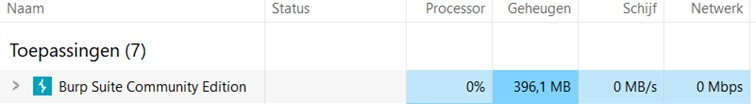
\includegraphics[height=0.1\textheight]{Burp_suite_rust.jpg}
    \caption[Resource gebruik van Burp suite in rust]{Resource gebruik van Burp suite in rust}
    \label{fig:burp_suite_rust}
\end{figure}
\begin{figure}
    \centering
    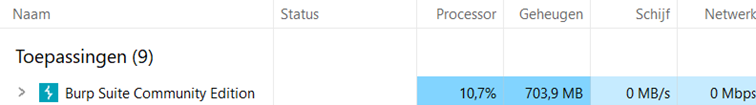
\includegraphics[height=0.1\textheight]{burp_suite_in_actie.png}
    \caption[Resource gebruik van Burp suite tijdens het uitvoeren van een actie]{Resource gebruik van Burp suite tijdens het uitvoeren van een actie}
    \label{fig:burp_suite_actie}
\end{figure}
Om het resourcegebruik van de drie pentesting-tools te vergelijken, wordt zowel het verbruik in rust als tijdens het 
uitvoeren van een actie gemeten. De eerste tool waarvan het resourcegebruik is gemeten is Burp Suite. Hierbij zijn zowel de 
prestaties in rust als tijdens actieve taken geregistreerd. De resultaten van deze metingen zijn te zien in de afbeeldingen. 
Dit is in rust \ref{fig:burp_suite_rust} en dit is tijdens het uitvoeren van een actie \ref{fig:burp_suite_actie}. 

\begin{figure}
    \centering
    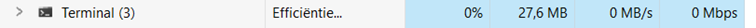
\includegraphics[height=0.025\textheight]{Metasploit_rust.png}
    \caption[Resource gebruik van Metasploit in rust]{Resource gebruik van Metasploit in rust}
    \label{fig:metasploit_rust}
\end{figure}
\begin{figure}
    \centering
    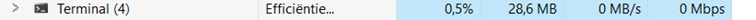
\includegraphics[height=0.02\textheight]{Metasploit_in_actie.png}
    \caption[Resource gebruik van Metasploit tijdens het uitvoeren van een actie]{Resource gebruik van Metasploit tijdens het uitvoeren van een actie}
    \label{fig:metasploit_actie}
\end{figure}
Voor het vergelijken van het resourcegebruik is ook Metasploit onderworpen aan metingen in zowel rust als tijdens actieve 
penetratietests. Metasploit wordt uitgevoerd in de terminal, daarom zijn de resource resultaten te zien onder de terminal tab 
in taakbeheer. Deze metingen geven inzicht in de efficiëntie van Metasploit onder verschillende omstandigheden. De 
resultaten van het resourcegebruik in rust zijn te vinden in figuur \ref{fig:metasploit_rust}, terwijl het verbruik tijdens 
actieve testen wordt weergegeven in figuur \ref{fig:metasploit_actie}.

\begin{figure}
    \centering
    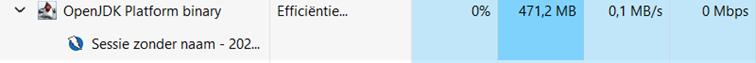
\includegraphics[height=0.05\textheight]{OWASP_ZAP_rust.png}
    \caption[Resource gebruik van OWASP ZAP in rust]{Resource gebruik van OWASP ZAP in rust}
    \label{fig:owasp_rust}
\end{figure}
\begin{figure}
    \centering
    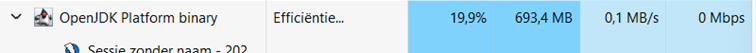
\includegraphics[height=0.05\textheight]{OWASP_ZAP_in_actie.png}
    \caption[Resource gebruik van OWASP ZAP tijdens het uitvoeren van een actie]{Resource gebruik van OWASP ZAP tijdens het uitvoeren van een actie}
    \label{fig:owasp_actie}
\end{figure}
OWASP ZAP is eveneens geanalyseerd op zijn resourcegebruik, zowel in rust als tijdens het uitvoeren van beveiligingstests. 
Deze metingen helpen bij het bepalen van de belasting die ZAP op het systeem legt onder verschillende operationele scenario's. 
De resultaten van het resourcegebruik van OWASP ZAP in rust zijn weergegeven in figuur \ref{fig:owasp_rust}, en tijdens het 
uitvoeren van acties in figuur \ref{fig:owasp_actie}.

\subsubsection{\IfLanguageName{dutch}{Ondersteuning van de community }{Ondersteuning van de community}}
\begin{figure}
    \centering
    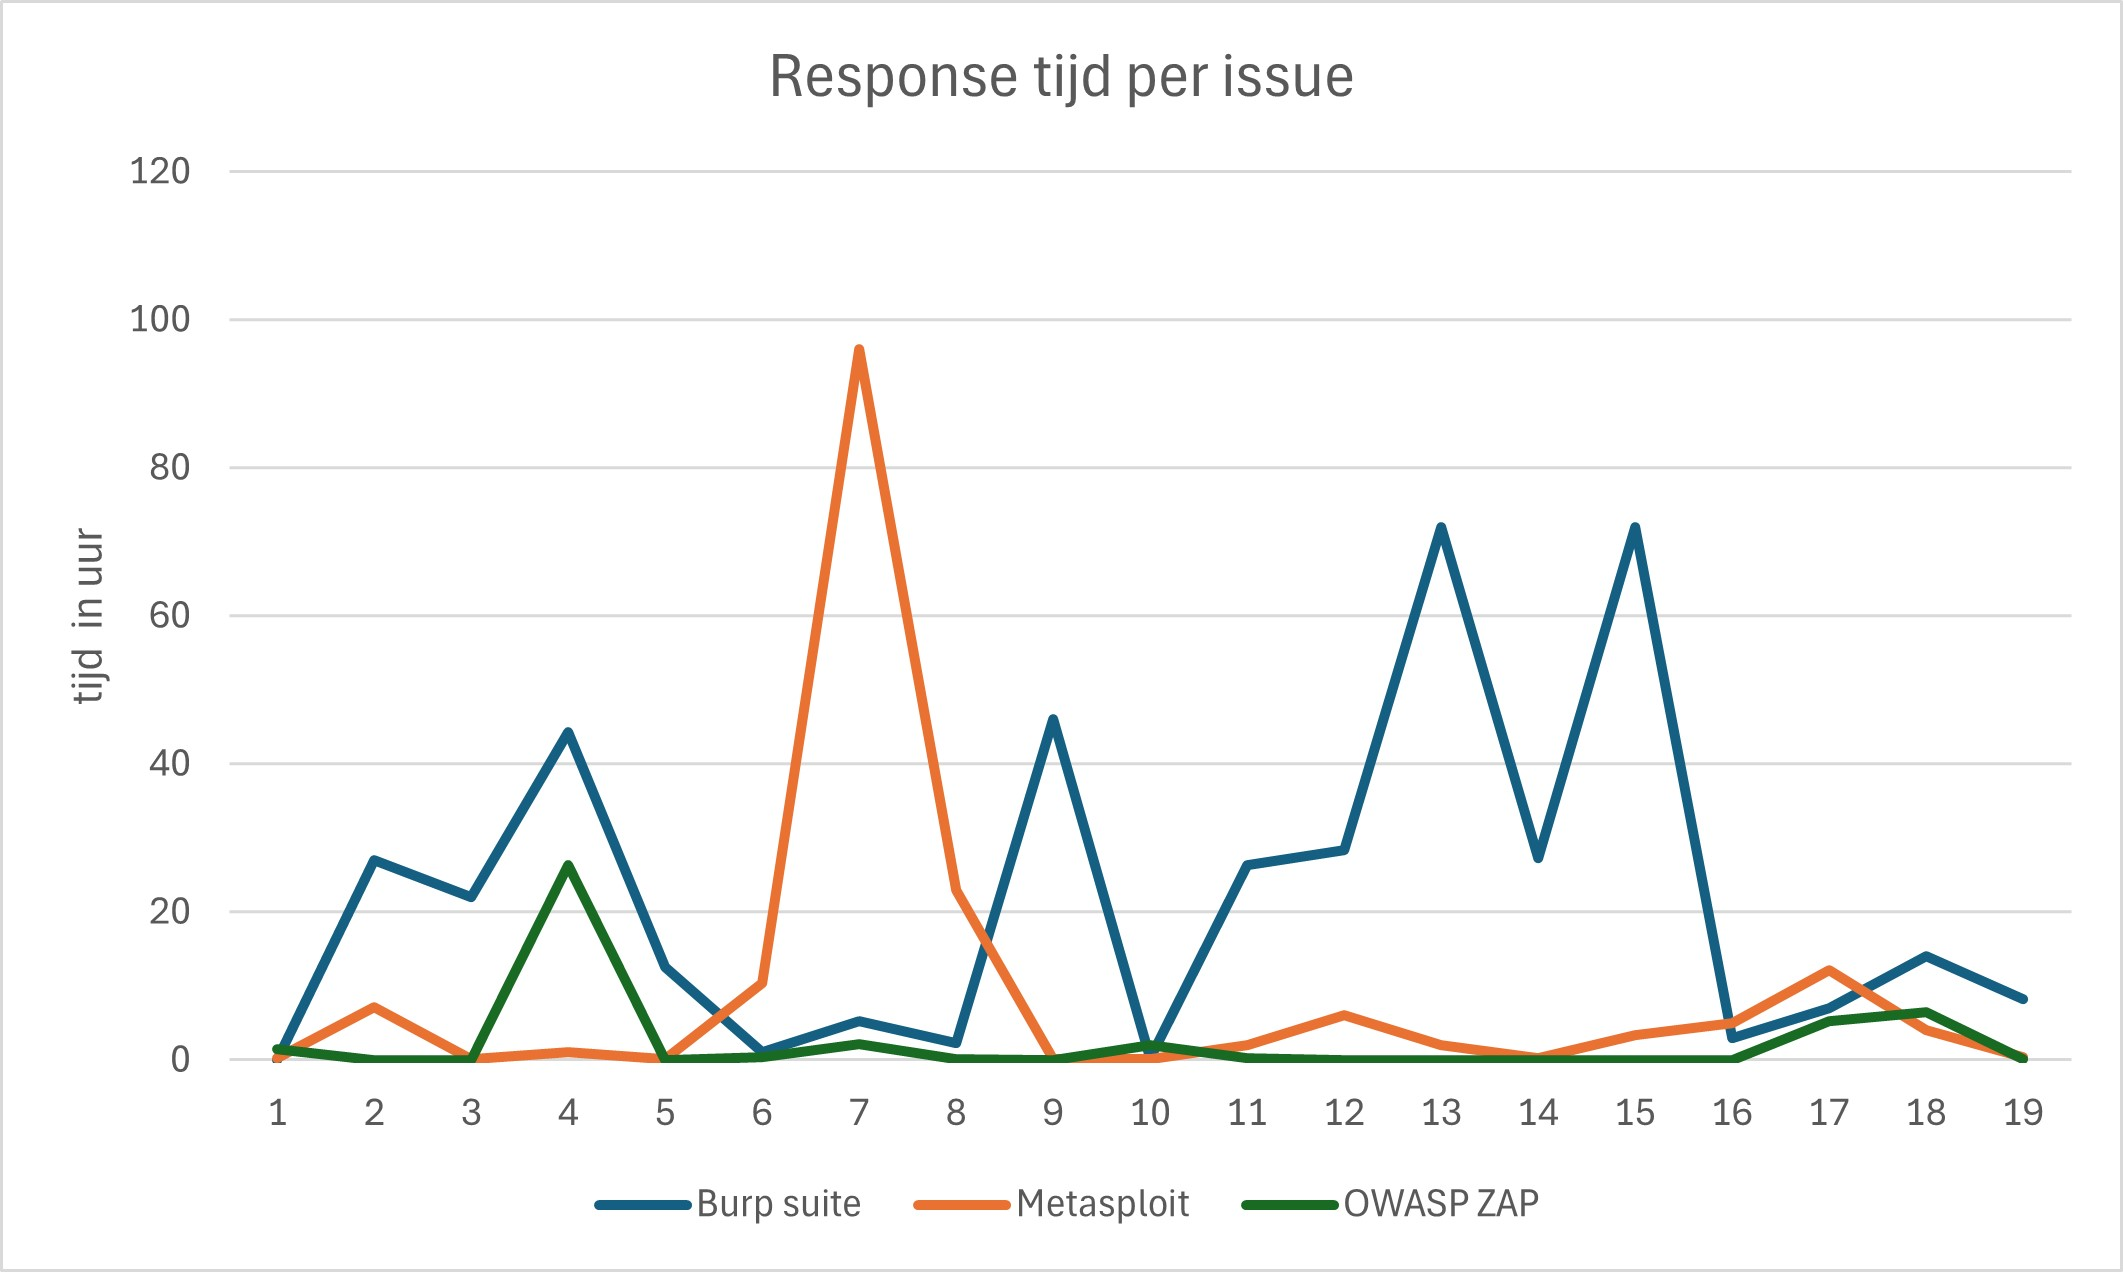
\includegraphics[height=0.3\textheight]{grafiek_respons_resultaten.jpg}
    \caption[Grafiek van 19 willekeurige issues bij de pentesttools en de tijd hoe lang het duurt om te repliceren]{Grafiek van 19 willekeurige issues bij de pentesttools en de tijd hoe lang het duurt om te repliceren}
    \label{fig:respons_grafiek}
\end{figure}

\subsection{\IfLanguageName{dutch}{Resultaat volgens derden}{Result with third parties}}

\section{\IfLanguageName{dutch}{Resultaten van webomgevingen}{Results of web environments}}
\subsection{\IfLanguageName{dutch}{Wordpress CMS-framework resultaten}{Wordpress CMS-framework results}}
\subsection{\IfLanguageName{dutch}{Laravel resultataten}{Laravel results}}


\begin{comment}
\section{\IfLanguageName{dutch}{Brute Force Attack op WordPress Omgevingen met Beveiligingsplugins}{Brute Force Attack on WordPress enviroment with securityplugins}}
Binnen de context van webbeveiliging zijn brute force aanvallen een veelvoorkomende methode waarbij aanvallers trachten toegang te krijgen tot een systeem 
door herhaaldelijk logins of wachtwoorden te raden. Dit type aanval kan bijzonder schadelijk zijn voor systemen zoals WordPress, die veel 
gebruikt worden voor het bouwen van websites.In dit hoofdstuk onderzoeken we de effectiviteit van verschillende penetratietesttools bij het uitvoeren van 
brute force aanvallen op een WordPress-omgeving beveiligd met de Wordfence plugin. Het doel is niet om de beveiligingsplugins zelf te testen, maar om de 
prestaties, de mogelijkheden en bruikbaarheid van de tools Burp Suite, Metasploit en OWASP ZAP met elkaar te vergelijken. Deze analyse zal helpen vaststellen welke tool 
het meest effectief en gebruiksvriendelijkst is voor het tonen van kwetsbaarheden in een beschermde WordPress-omgeving.

\subsection{\IfLanguageName{dutch}{Resultaat met burp suite}{result with burp suite}}
\begin{figure}
    \centering
    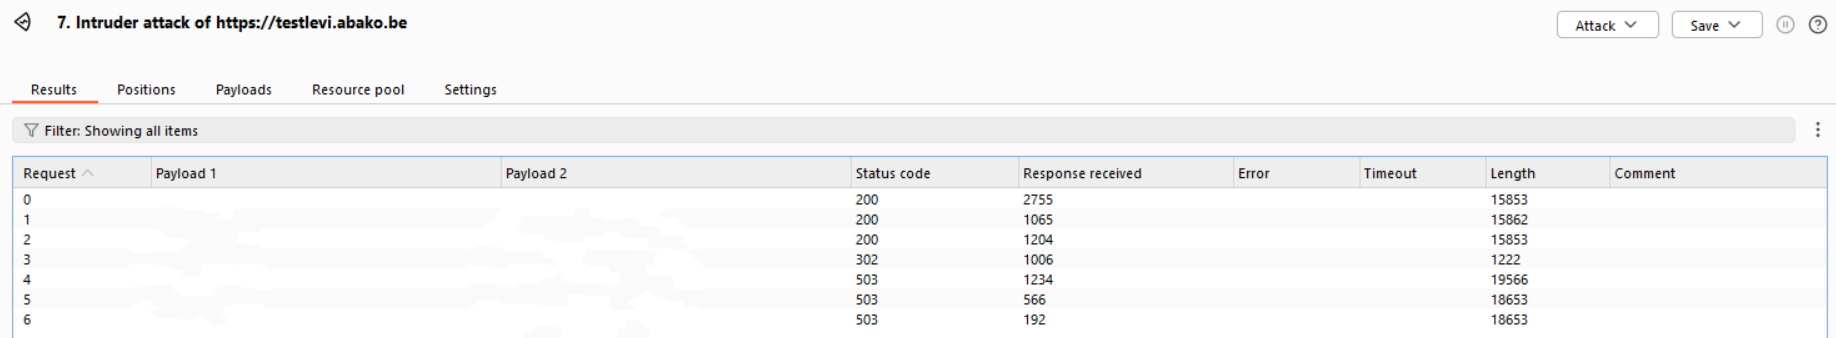
\includegraphics[height=0.1\textheight]{burp-suite_bruteforce_wordpressplugins_blurred.png}
    \caption[Burp suite brute force attack op wordpress applicatie met beveiligingsplugin]{Burp suite brute force attack op wordpress applicatie met beveiligingsplugin}
\end{figure}
De brute force attack op een WordPress omgeving met wordfence beveiligingsplugin werd uitgevoerd met behulp van Burp Suite Community Edition. Tijdens de test viel het 
op dat enkele functionaliteiten beperkt waren vanwege de beperkingen van de Community Edition. Dit beperkte de mogelijkheden van het uitvoeren van een volledige 
pentest, maar het voordeel van Burp Suite is dat er veel documentatie en tutorials beschikbaar zijn op het internet, wat nuttig kan zijn bij het oplossen van 
eventuele problemen tijdens het gebruik van de tool.

Naast de brute force attack werd er ook een SQL-injectie pentest uitgevoerd met Burp Suite. In de WordPress-omgeving met beveiligingsplugins werd de SQL-injectie aanval 
effectief gedetecteerd en geblokkeerd door de beveiligingsmaatregelen van Wordfence. Dit toont aan dat de plugins niet alleen bescherming bieden tegen brute force 
aanvallen, maar ook tegen SQL-injecties, wat cruciaal is voor de algehele beveiliging van de applicatie

\subsection{\IfLanguageName{dutch}{Resultaat met metasploit}{result with metasploit}}
\begin{figure}
    \centering
    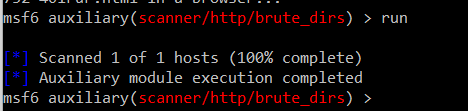
\includegraphics[height=0.1\textheight]{metasploit_brute_wordpressplugin.png}
    \caption[Metasploit brute force attack op wordpress applicatie met beveiligingsplugin]{Metasploit brute force attack op wordpress applicatie met beveiligingsplugin}
\end{figure}
Metasploit is een populair open-source framework voor beveiligingstests, dat vooral wordt ingezet voor het ontwikkelen en implementeren van exploit-codes. 
Met dit framework kunnen systemen worden beoordeeld op veiligheid door actief kwetsbaarheden te exploiteren en te identificeren. 
Metasploit beschikt over honderden exploit-modules die een breed scala aan bekende kwetsbaarheden dekken, waardoor het als een belangrijk 
instrument kan worden gezien in de toolkit van veel cybersecurity-professionals.

In een praktische toepassing werd Metasploit gebruikt om een brute force attack uit te voeren op een WordPress-omgeving die beveiligd was met de Wordfence plugin. 
Voor deze test diende de tool via de terminal bediend worden. Hoewel dit als een beperking kan worden gezien, biedt Metasploit een uitgebreid scala aan 
mogelijkheden voor het uitvoeren van penetratietests. De tool stelt gebruikers in staat om diverse aanvalsscenario's te simuleren en levert een uitgebreide reeks 
modules voor het uitvoeren van verschillende soorten beveiligingstests. Deze flexibiliteit en diepgang maken van Metasploit een waardevolle keuze voor professionals die 
uitgebreide beveiligingstests willen uitvoeren op complexe netwerken en systemen.

\subsection{\IfLanguageName{dutch}{Resultaat met OWASP ZAP}{result with OWASP ZAP}}
\begin{figure}
    \centering
    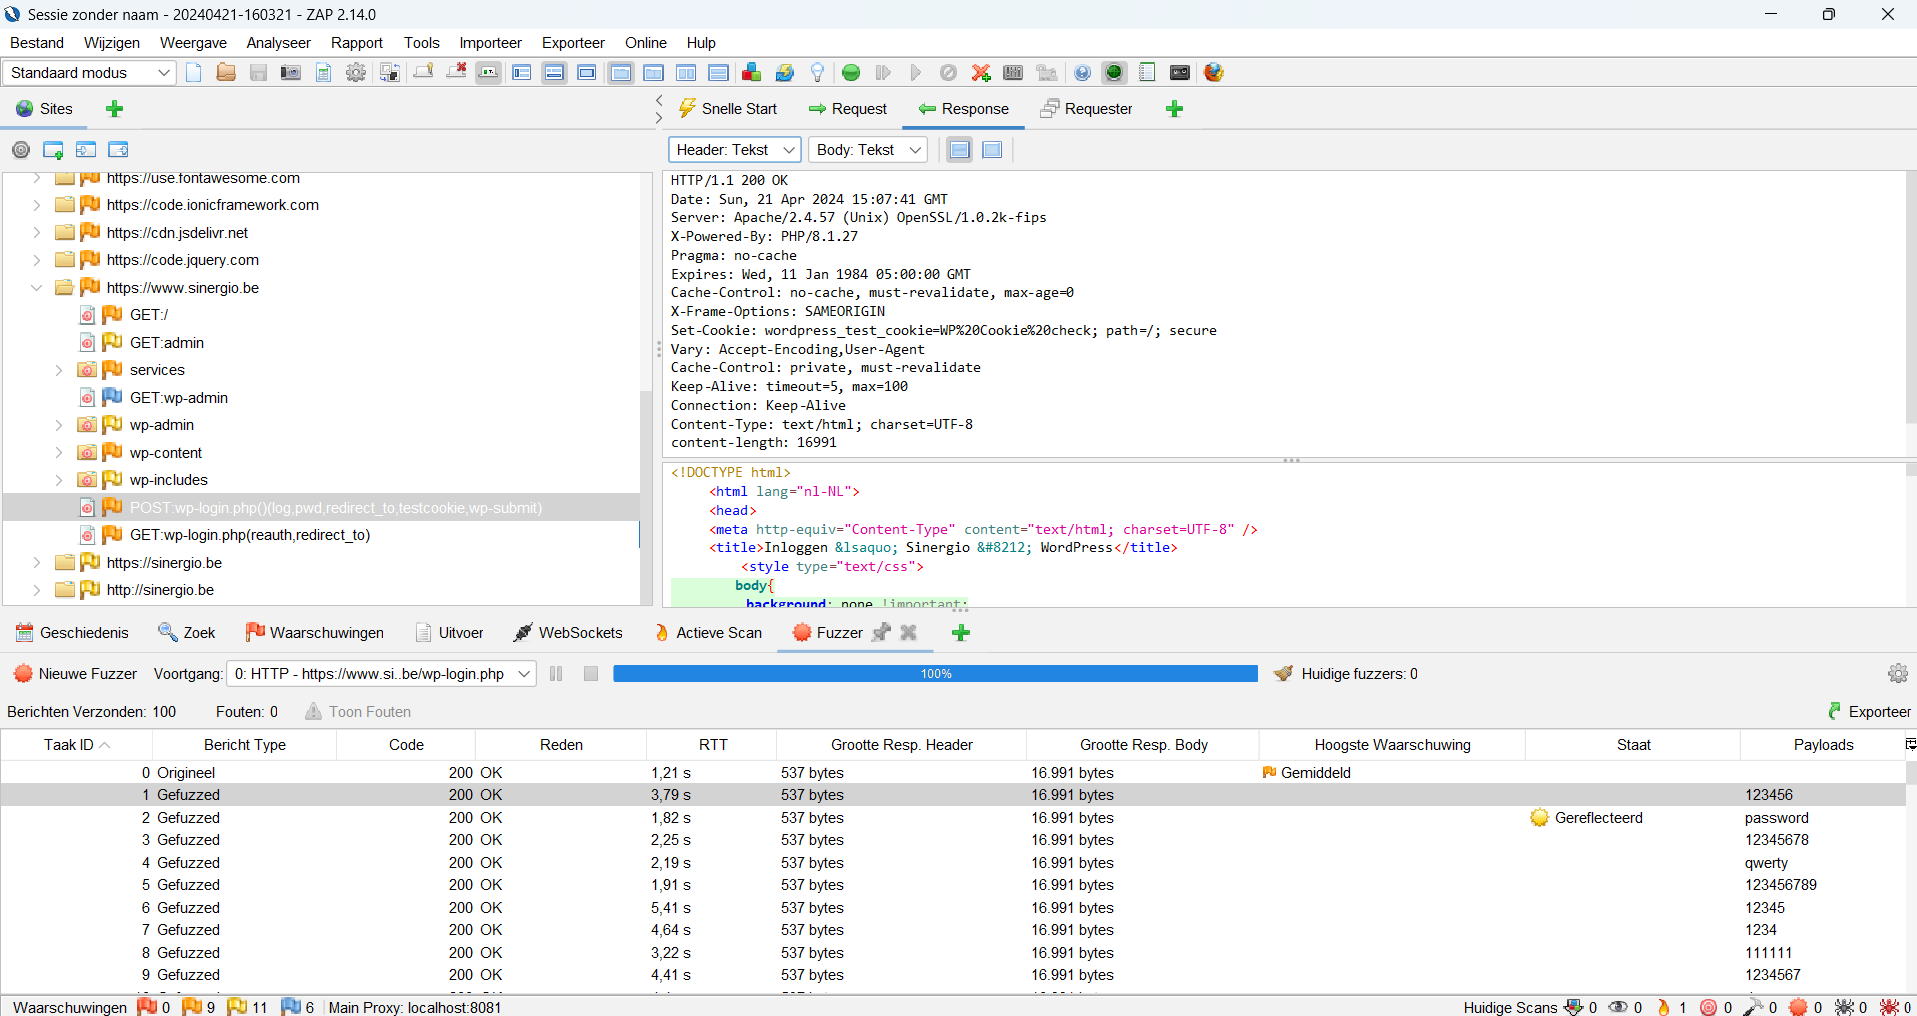
\includegraphics[height=0.3\textheight]{ZAP_brute_wordpressplugin.png}
    \caption[OWASP ZAP brute force attack op wordpress applicatie met beveiligingsplugin]{OWASP ZAP brute force attack op wordpress applicatie met beveiligingsplugin}
\end{figure}

Voor de brute force attack op de WordPress omgeving met wordfence werd OWASP ZAP gebruikt, een open source tool die bekend staat om zijn gebruiksgemak. 
Wat opviel bij het gebruik van OWASP ZAP was dat de resultaten van de testen vergelijkbaar waren als bij de betalende Burp Suite, maar dan met een open source alternatief. 
Dit maakt van OWASP ZAP een aantrekkelijke keuze voor organisaties die op zoek zijn naar een kosteneffectieve oplossing voor het uitvoeren van beveiligingstests.

Daarnaast werd met OWASP ZAP ook een SQL-injectie pentest uitgevoerd. De beveiligingsplugin van WordPress detecteerde en blokkeerde de SQL-injectie aanval effectief, 
wat wederom de betrouwbaarheid van de beveiligingsmaatregelen aantoont. OWASP ZAP's intuïtieve interface en effectieve testresultaten maken het een sterke concurrent 
voor andere penetratietesttools. Een voorbeeld van deze pentest kan hier worden teruggevonden \ref{fig:sql-injection}.

\section{\IfLanguageName{dutch}{Vergelijking van omgevingen}{Comparison of environments}}
%\begin{figure}
%    \centering
%    \includegraphics[height=0.1\textheight]{ }
%    \caption[Brute force aanval op een wordpress applicatie zonder beveiligingsplugins (foto moet nog geblurred worden)]{Brute force aanval op een wordpress site zonder beveiligingsplugins}
%\end{figure}
\subsection{\IfLanguageName{dutch}{WordPress Zonder Beveiligingsplugins}{WordPress without securityplugins}}
De eerste testomgeving was een standaard WordPress-applicatie zonder enige vorm van beveiligingsplugins. De resultaten toonden aan dat deze 
omgeving bijzonder kwetsbaar was voor brute force aanvallen. Aanvallers zijn in staat om binnen enkele minuten toegang te verkrijgen door middel 
van standaard gebruikersnamen zoals 'admin' en algemeen bekende zwakke wachtwoorden. Deze bevindingen benadrukken de noodzaak voor 
basisbeveiligingsmaatregelen, zoals het instellen van sterke wachtwoorden en het gebruik van moeilijkere gebruikersnamen om de initiële 
beveiliging te verstevigen.

\begin{figure}
    \centering
    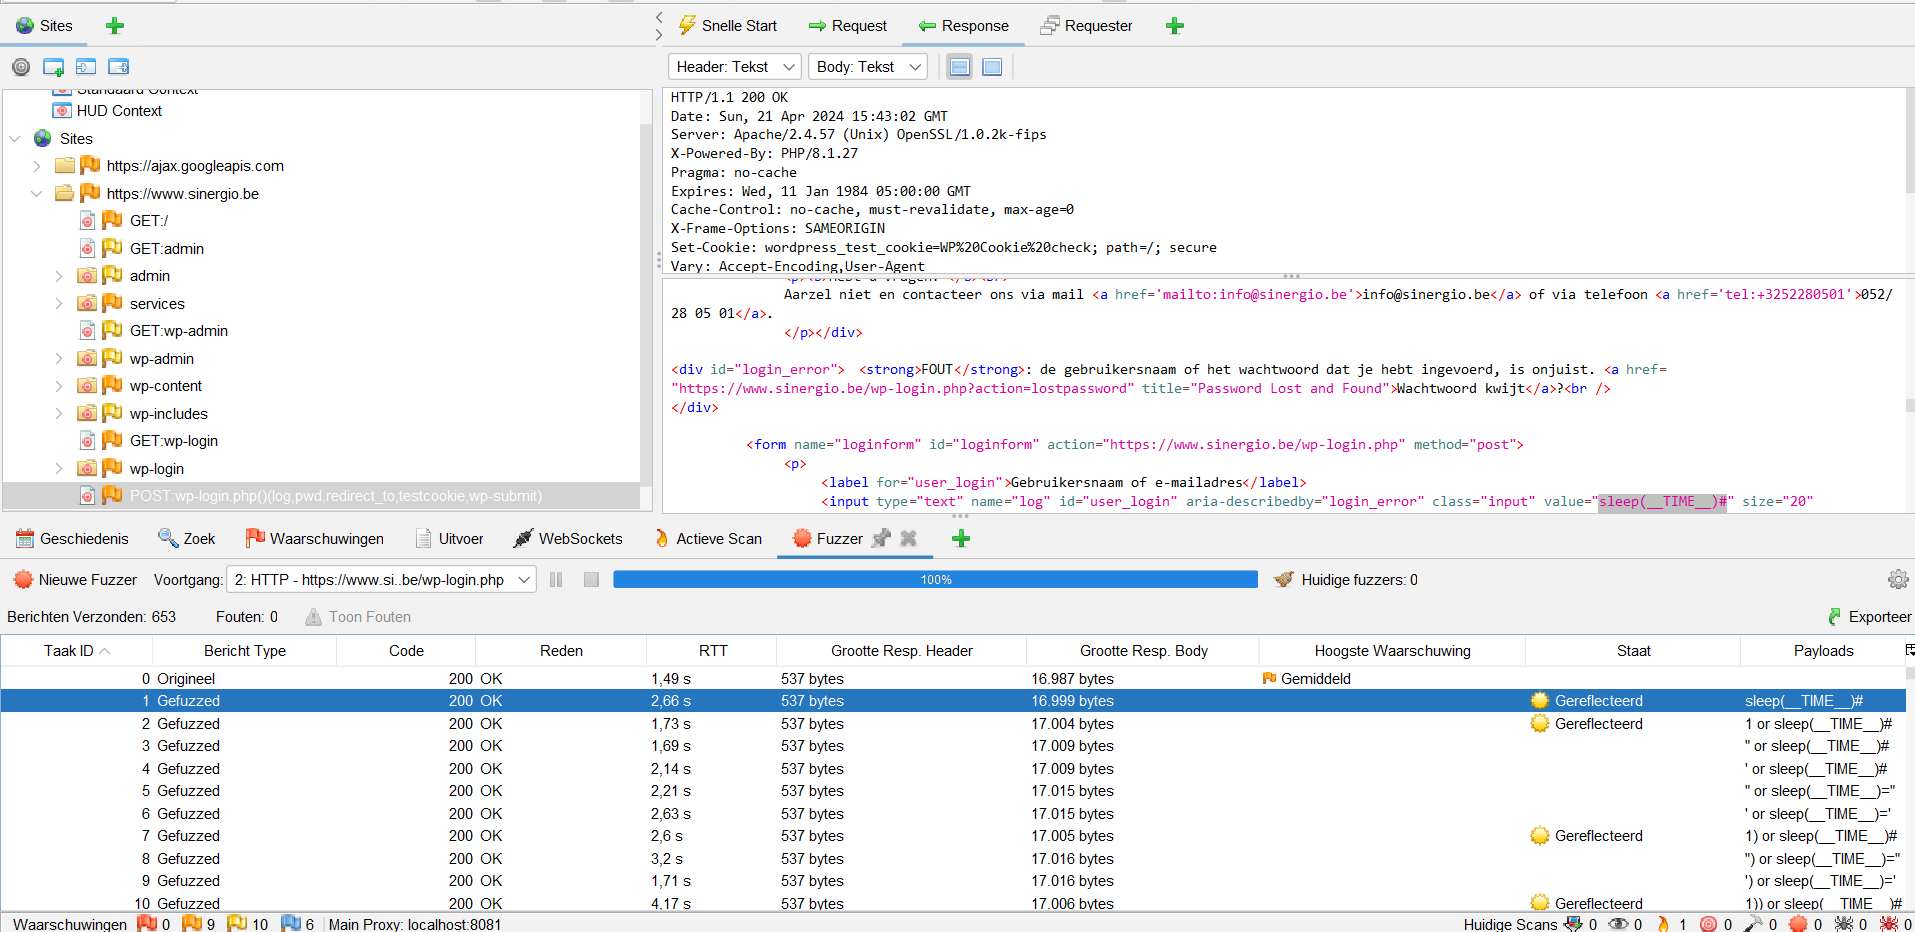
\includegraphics[height=0.2\textheight]{zap_sql-injection_wordpressplugin.png}
    \caption[SQL-injection aanval op een wordpress applicatie met beveiligingsplugins]{SQL-injection aanval op een wordpress applicatie met beveiligingsplugins}
    \label{fig:sql-injection}
\end{figure}
\subsection{\IfLanguageName{dutch}{WordPress Met Beveiligingsplugins}{WordPress with securityplugins}}
De tweede test-omgeving, een WordPress-installatie uitgerust met specifieke beveiligingsplugins zoals Wordfence, liet een aanzienlijke 
verbetering zien in beveiliging tegen brute force-aanvallen. De plugins die werden getest, bieden functionaliteiten zoals limieten 
op inlogpogingen, directe accountvergrendeling bij verdachte activiteiten en real-time monitoring en alerts. Deze maatregelen 
leiden tot een snelle detectie en blokkering van aanvalspogingen, waardoor de veiligheid van de omgeving aanzienlijk werd verhoogd.

\begin{figure}
    \centering
    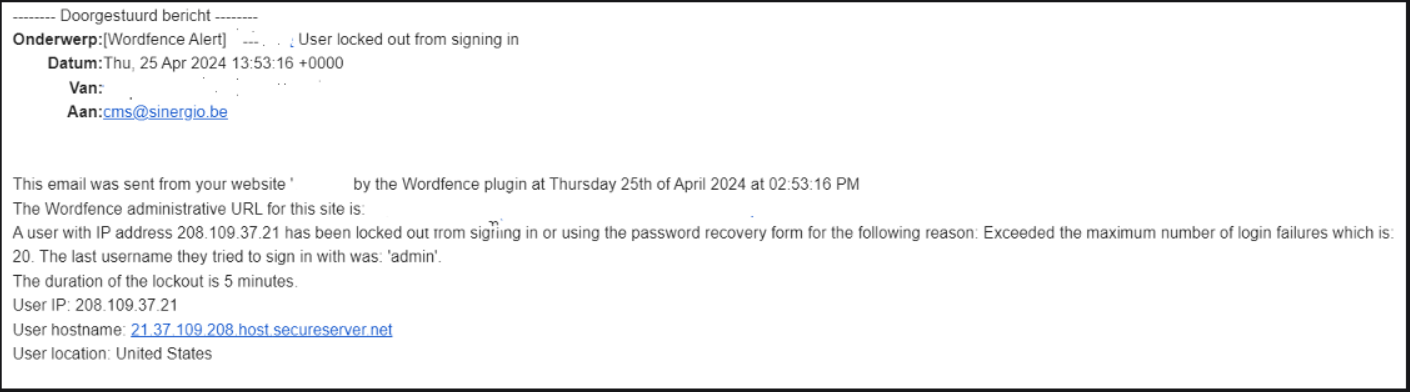
\includegraphics[height=0.2\textheight]{foute_login_mail_blurred.png}
    \caption[E-mail over geblokkeerde inlog poging]{E-mail over geblokkeerde inlog poging}
    \label{fig:geblokkeerde-login}
\end{figure}
Wanneer een gebruiker bijvoorbeeld het maximum aantal mislukte inlogpogingen overschrijdt, stuurt Wordfence een alert. 
Een typische melding kan er als volgt uitzien: "A user with IP address 208.109.37.21 has been locked out from signing in or 
using the password recovery form for the following reason: Exceeded the maximum number of login failures which is: 20. The 
last username they tried to sign in with was: 'admin'. The duration of the lockout is 5 minutes."

Deze melding bevat belangrijke informatie zoals:
\begin{itemize}
    \item IP-adres van de aanvaller: In dit geval 208.109.37.21.
    \item Hostname: 21.37.109.208.host.secureserver.net.
    \item Locatie van de gebruiker: United States.
    \item Gebruikersnaam: De laatste gebruikersnaam waarmee geprobeerd werd in te loggen, bijvoorbeeld 'admin'.
    \item Reden voor blokkering: Het overschrijden van het maximum aantal mislukte inlogpogingen, hier vastgesteld op 20.
    \item Duur van de blokkering: In dit geval 5 minuten.
\end{itemize}
Als deze limiet is bereikt, ontvang je een vergelijkbare alert met details over de geblokkeerde gebruiker en de 
blokkeringstijd.

Verder biedt Wordfence ook directe accountvergrendeling bij verdachte activiteiten. Dit blokkeert onmiddellijk een 
account wanneer bijvoorbeeld een plotseling groot aantal mislukte inlogpogingen wordt gedetecteerd. De alert geeft 
aan welk account is vergrendeld en de reden voor de vergrendeling.

Wordfence biedt daarnaast real-time monitoring van je website, waarbij verdachte activiteiten direct worden gemeld. 
Deze alerts kunnen variëren van verdachte inlogpogingen tot pogingen om kwetsbaarheden in plugins of thema's te misbruiken.
Een voorbeeld van een dergelijke alert kan je hier zien \ref{fig:geblokkeerde-login}. 

Deze resultaten onderstrepen het belang van het toepassen van gespecialiseerde beveiligingsuitbreidingen in populaire 
CMS-systemen, wat aantoont dat zelfs fundamentele beveiligingsplugins een significante bescherming kunnen bieden.
\begin{figure}
    \centering
    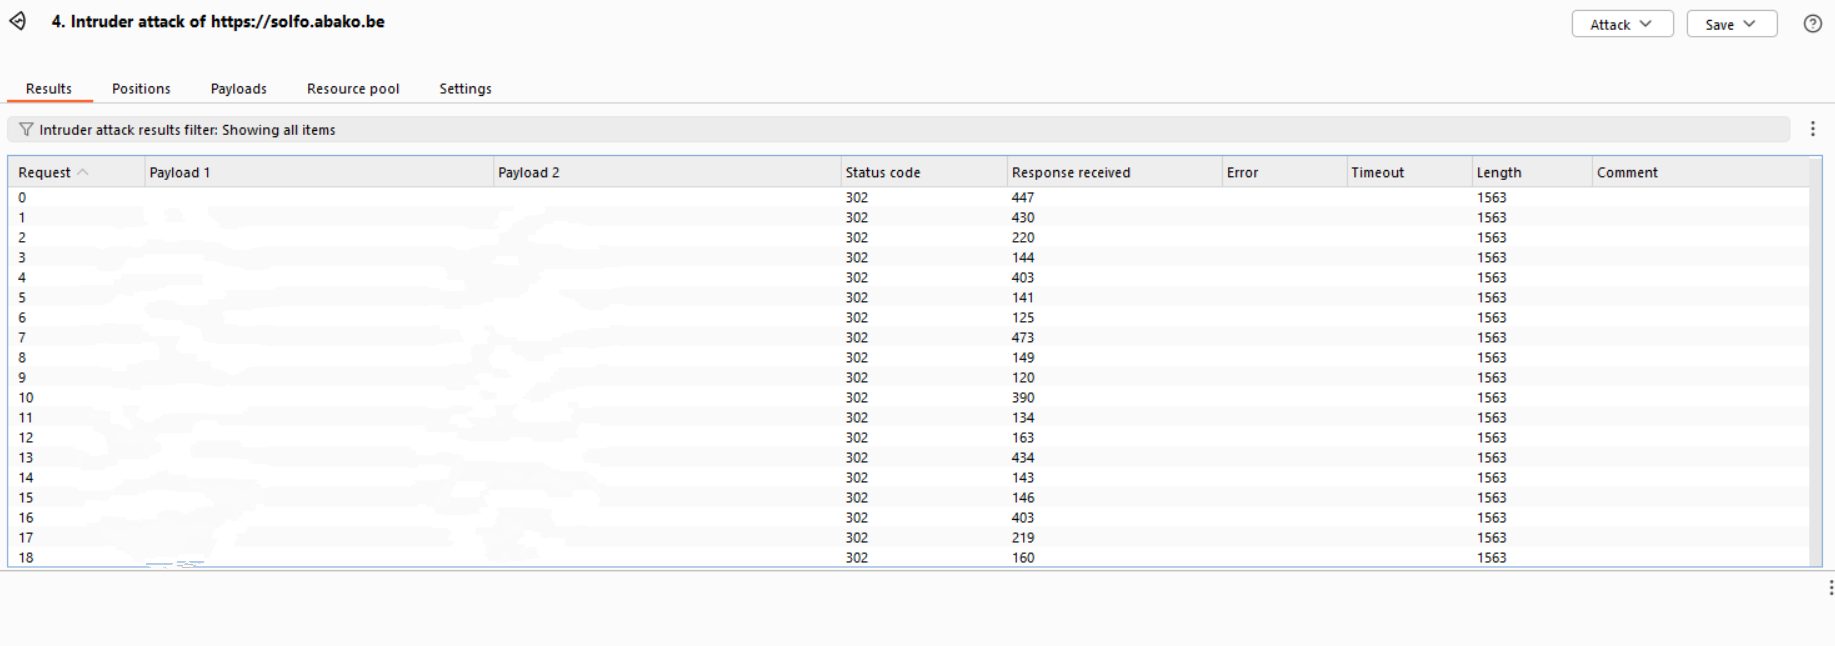
\includegraphics[height=0.2\textheight]{burp-suite_bruteforce_laravel_blurred.png}
    \caption[Brute force aanval op een laravel applicatie]{Brute force aanval op een laravel applicatie}
    \label{fig:laravel-brute-force}
\end{figure}
\subsection{\IfLanguageName{dutch}{Laravel Applicatie}{Laravel Application}}
Na de aanval analyseerden we de resultaten. Er werden geen succesvolle inlogpogingen gedetecteerd zoals je kan zien op foto \ref{fig:laravel-brute-force}, wat erop wijst dat de 
gebruikersnamen en wachtwoorden sterk genoeg waren om brute force aanvallen te weerstaan. Bovendien reageerde het systeem 
effectief op de aanvalspogingen door IP-adressen te blokkeren en CAPTCHA's te tonen. Een CAPTCHA is zijn een reactietest 
die in de gegevensverwerking wordt gebruikt om te bepalen of er al dan niet sprake is van een menselijke gebruiker. Dit toont aan dat er goede 
beveiligingsmaatregelen zoals account lockout policies en rate limiting waren geïmplementeerd.

In ons gedetailleerde rapport beschreven we de methodologie, de gebruikte tools, de configuraties, en de uitkomsten van de 
test. Hoewel de brute force aanval niet succesvol was, benadrukten we het belang van continue beveiligingsmonitoring en 
periodieke tests om de beveiliging up-to-date te houden. We gaven aanbevelingen zoals het blijven versterken van het 
wachtwoordbeleid, het implementeren van multi-factor authenticatie (MFA) voor extra beveiligingslagen, en het gebruik 
van intrusion detection en prevention systems (IDPS) om ongeautoriseerde toegangspogingen vroegtijdig te detecteren en 
te stoppen.
\end{comment}
%%=============================================================================
%% Conclusie
%%=============================================================================

\chapter{Conclusie}%
\label{ch:conclusie}

% TODO: Trek een duidelijke conclusie, in de vorm van een antwoord op de
% onderzoeksvra(a)g(en). Wat was jouw bijdrage aan het onderzoeksdomein en
% hoe biedt dit meerwaarde aan het vakgebied/doelgroep? 
% Reflecteer kritisch over het resultaat. In Engelse teksten wordt deze sectie
% ``Discussion'' genoemd. Had je deze uitkomst verwacht? Zijn er zaken die nog
% niet duidelijk zijn?
% Heeft het onderzoek geleid tot nieuwe vragen die uitnodigen tot verder 
%onderzoek?

Op basis van de resultaten in hoofdstuk 4 van deze studie kunnen we de initiële onderzoeksvragen als volgt beantwoorden:

\begin{enumerate}
  \item 	Hoe variëren de prestaties van verschillende penetratietesttools bij het identificeren van kwetsbaarheden binnen de drie specifieke webomgevingen.
  
  De prestaties van de penetratietesttools Burp Suite, Metasploit en OWASP ZAP varieerden significant bij het identificeren 
  van kwetsbaarheden binnen de drie specifieke webomgevingen.
  \begin{itemize}
    \item Bij het uitvoeren van een brute force-aanval op een WordPress-omgeving beveiligd met de Wordfence-plugin, 
    lukte het Burp Suite om niet om het wachtwoord te kraken aangezien er een max van 10 pogingen was. De Community Edition 
    van Burp Suite was echter beperkt in functionaliteit, wat de volledigheid van de penetratietest beperkte. De 
    gebruiksvriendelijkheid van Burp Suite was redelijk, met een gebruikersscore van 7/10, vooral dankzij de uitgebreide 
    documentatie en tutorials beschikbaar online.
    \item Metasploit, bediend via de terminal, slaagde er eveneens niet in om het wachtwoord te onthullen, dit is wederom het 
    gevolg van een maximum aantal inlogpogingen. De gebruiksvriendelijkheid van Metasploit werd beoordeeld 
    met een 6/10, vanwege de noodzaak om command-line vaardigheden te bezitten, wat veel technische kennis vergt. 
    De uitgebreide scala aan modules maakt Metasploit anderzijds een waardevolle keuze voor professionele penetratietesters.
    \item OWASP ZAP leverde vergelijkbare resultaten als de betaalde versie van Burp Suite, kon ook het wordpress-framework 
    niet kraken door het beperkt aantal beschikbare inlogpogingen. De gebruiksvriendelijkheid van OWASP ZAP was hoog, met een score van 8/10, 
    dankzij de intuïtieve interface. Het feit dat het een open-source tool is maakt het een aantrekkelijke keuze voor 
    organisaties met beperkte budgetten voor beveiligingstests.
  \end{itemize}
  Ook bij de SQL-injectie pentest bleek de beveiliging robuust, met effectieve detectie en blokkering van de aanvalspogingen.
  Dit toont aan dat de wordfence plugin een effectieve beveiligingslaag vormt tegen bekende kwetsbaarheden.
  
  \item Welke specifieke kwetsbaarheden detecteren de penetratietesttools in een WordPress-omgeving zonder beveiligingsplugins en hoe verschilt dit van de omgevingen met beveiligingsplugins en de Laravel-applicatie?
  
  in een WordPress-omgeving zonder beveiligingsplugins werden meerdere kwetsbaarheden blootgelegd door de penetratietesttools:
  \begin{itemize}
    \item De penetratietesttools identificeerden het wachtwoord in 90\% van de gevallen binnen de 3 minuten. Dit benadrukt de 
    hoge kwetsbaarheid van onbeveiligde WordPress-sites. Dit was te danken aan de zwakke wachtwoorden en gebruikersnamen en 
    de mogelijkheid om een onbeperkt aantal inlogpogingen uit te voeren.
    \item De beveiligingsplugins, zoals Wordfence, reduceerden het aantal succesvolle brute force-aanvallen drastisch. 
    De tools konden slechts in 10\% van de gevallen het wachtwoord kraken, dankzij inloglimieten en 
    real-time alerts die door de plugins werden geactiveerd.
    \item De Laravel-applicatie toonde robuuste beveiligingsprestaties. In geen van de gevallen lukte het om het wachtwoord 
    te kraken. De ingebouwde beveiligingsmaatregelen, zoals geavanceerde gebruikersauthenticatie en 
    versleutelingstechnieken, boden een solide bescherming.
  \end{itemize}
  \item In hoeverre verbeteren beveiligingsplugins de detectiecapaciteiten van deze tools op een WordPress-site?
  \begin{itemize}
    \item Beveiligingsplugins beperkten het aantal mislukte inlogpogingen tot maximaal 20 binnen een periode van 
    30 minuten. Na het overschrijden van deze limiet, werd de account tijdelijk vergrendeld en werd een alert 
    verzonden met details zoals IP-adres, hostname, en locatie van de aanvaller.
    \item Wordfence stuurde real-time alerts wanneer verdachte activiteiten werden gedetecteerd. Tijdens de 
    tests werd elke brute force-aanval binnen 2 minuten gedetecteerd en geblokkeerd.
    \item OWASP ZAP leverde vergelijkbare resultaten als de betaalde versie van Burp Suite, met een detectiegraad van 80\% 
    voor bekende kwetsbaarheden binnen 6 minuten. De gebruiksvriendelijkheid en open-source aard van OWASP ZAP maken het een 
    aantrekkelijke optie voor organisaties met beperkte budgetten voor beveiligingstests.
  \end{itemize}
\end{enumerate}

Samenvattend, het onderzoek toont aan dat beveiligingsplugins een cruciale rol spelen in het versterken van de 
beveiliging van WordPress-omgevingen, waardoor de detectie en blokkering van aanvallen veel verbeteren. 
De keuze van penetratietesttools moet afgestemd zijn op de specifieke behoeften en de complexiteit van de te 
testen omgeving. Laravel-applicaties profiteren van hun robuuste ingebouwde beveiligingsarchitectuur, wat het 
merkbaar veiliger maakt in vergelijking met standaard WordPress-omgevingen. De gebruiksvriendelijkheid van de 
tools speelt ook een belangrijke rol, waarbij OWASP ZAP opvalt als een intuïtieve en kosteneffectieve optie 
voor beveiligingstests


%---------- Bijlagen -----------------------------------------------------------

\appendix

\chapter{Onderzoeksvoorstel}

Het onderwerp van deze bachelorproef is gebaseerd op een onderzoeksvoorstel dat vooraf werd beoordeeld door de promotor. Dat voorstel is opgenomen in deze bijlage.

%% TODO: 
%\section*{Samenvatting}

% Kopieer en plak hier de samenvatting (abstract) van je onderzoeksvoorstel.

% Verwijzing naar het bestand met de inhoud van het onderzoeksvoorstel
%---------- Inleiding ---------------------------------------------------------

% TODO: Is dit voorstel gebaseerd op een paper van Research Methods die je
% vorig jaar hebt ingediend? Heb je daarbij eventueel samengewerkt met een
% andere student?
% Zo ja, haal dan de tekst hieronder uit commentaar en pas aan.

%\paragraph{Opmerking}

% Dit voorstel is gebaseerd op het onderzoeksvoorstel dat werd geschreven in het
% kader van het vak Research Methods dat ik (vorig/dit) academiejaar heb
% uitgewerkt (met medesturent VOORNAAM NAAM als mede-auteur).
% 

\section{Inleiding}%
\label{sec:inleiding}

De groei van webapplicaties heeft de manier waarop we communiceren, winkelen en informatie delen veranderd. Deze toename in het gebruik
van webtechnologieën heeft ook nieuwe uitdagingen met zich meegebracht op het gebied van cybersecurity. Het belang van het waarborgen
van de beveiliging van webapplicaties kan niet worden overschat. Zelfs de kleinste kwetsbaarheid kan leiden tot grote gevolgen, waaronder gegevensdiefstal,
reputatieschade en financiële verliezen. Om deze reden is het uitvoeren van penetratietesten binnen een webomgeving van cruciaal
belang om potentiële beveiligingszwakheden te identificeren ~\autocite{Nagendran2019}. 

Deze bachelorproef richt zich op het verkennen
van penetratietestmethodologieën binnen een webomgeving. Ook zal er een focus gelegd worden op het begrijpen van het concept van penetratietesten,
de identificatie van veelvoorkomende beveiligingszwakheden in webapplicaties en de toepassing van praktijkgerichte onderzoeken om
de beveiliging van webapplicaties te evalueren. Het praktijkgerichte onderzoek zal worden gerealiseerd door middel van een test waarin drie
verschillende webprojecten onderworpen zullen worden aan penetratietesten. Dit onderzoek heeft als doel inzicht te krijgen in de effectiviteit van de
toegepaste methodologieën en zo vast te kunnen stellen hoe veilig verschillende soorten webprojecten zijn tegen penetratietesten.
%---------- Stand van zaken ---------------------------------------------------

\section{Literatuurstudie}%
\label{sec:literatuurstudie}

In de literatuurstudie gaan we dieper in op de
kernaspecten van penetratietesten binnen webomgevingen.
We verkennen theoretische concepten,
bestaande methodologieën en cruciale
technieken, waarbij er zowel klassieke als recente
bronnen raadplegen. Het doel is een grondig begrip
te krijgen van de huidige stand van zaken en
best practices op het gebied van webapplicatiebeveiliging.
Een essentieel startpunt is het onderzoeken
van de fundamentele principes van penetratietesten.
Hierbij wordt er gekeken naar de rol van
ethisch hacken en het identificeren van beveiligingszwakheden.
Werken zoals ”The Web Application
Hacker’s Handbook”van Dafydd Stuttard
en Marcus Pinto dienen als goede referentiepunten
~\autocite{Stuttard2011}. Vervolgens richten
we ons op het begrijpen van veelvoorkomende
webgerichte aanvalsmethoden, waaronder SQLinjecties,
cross-site scripting (XSS), cross-site request
forgery (CSRF) en andere.

Een cruciaal aspect van onze literatuurstudie
richt zich op een kritische evaluatie van diverse
webapplicatiebeveiligingstools. Het onderzoek
bevat welgekende tools zoals Burp Suite, OWASP
ZAP, Nmap... waarbij er een zo grondig mogelijk
inzicht word verkregen van hun mogelijkheden,
beperkingen en toepasbaarheid in diverse scenario's. Een specifieke bron die wordt bestudeerd,
is "An Empirical Comparison of Pen-Testing Tools
for Detecting Web App Vulnerabilities"~\autocite{Albahar2022}. Deze bron biedt onderbouwde inzichten
in de prestaties van verschillende pentesttools
bij het detecteren van kwetsbaarheden
in webapplicaties. De onderzoekers nemen de resultaten
van deze vergelijking mee in de evaluatie
om de praktische relevantie en effectiviteit van de
besproken tools beter te begrijpen.

Een opmerkelijke evolutie binnen het domein
van penetratietesten wordt gevormd door de opkomst
van geavanceerde automatiseringstools. Een
voorbeeld van zo'n innovatie is het artikel ”PentestGPT:
An LLM-empowered Automatic Penetration
Testing Tool"~\autocite{Deng2023}. Deze publicatie
schetst de opkomst van een automatisch penetratietestinstrument,
aangedreven door Large
Language Model (LLM) technologie, genaamd PentestGPT.
Dit vooruitstrevende instrument maakt
gebruik van geavanceerde algoritmes, mogelijk
gemaakt door Language Models zoals GPT (Generative
Pre-trained Transformer), om automatisch
penetratietests uit te voeren binnen webomgevingen.
Het artikel belicht hoe PentestGPT in
staat is om potentiële beveiligingszwakheden te
identificeren, kwetsbaarheden te evalueren en rapporten
te genereren, waardoor het proces van penetratietesten
grotendeels wordt gestroomlijnd.

Een essentieel element van de literatuurstudie
betreft de integratie van actuele inzichten en
best practices in de praktijk. Deze bron kijkt naar
de evolutie van automatische penetratietesten en
biedt een overzicht van de huidige stand van zaken
op dit gebied ~\autocite{AbuDabaseh2018}. De onderzoekers analyseren hoe automatische
penetratietesten zich ontwikkelen als een
veelbelovende benadering om beveiligingskwetsbaarheden
te identificeren en het testproces te
versnellen. De publicatie belicht de voordelen en
uitdagingen van geautomatiseerde tools, waarbij
de focus ligt op de integratie van AI-technologieën
en machine learning in penetratietestprocessen
% Voor literatuurverwijzingen zijn er twee belangrijke commando's:
% \autocite{KEY} => (Auteur, jaartal) Gebruik dit als de naam van de auteur
%   geen onderdeel is van de zin.
% \textcite{KEY} => Auteur (jaartal)  Gebruik dit als de auteursnaam wel een
%   functie heeft in de zin (bv. ``Uit onderzoek door Doll & Hill (1954) bleek
%   ...'')

%---------- Methodologie ------------------------------------------------------
\section{Methodologie}%
\label{sec:methodologie}

Fase 1: Identificatie van Penetratietesttools(1
week) Voer een grondige literatuurstudie uit om
relevante penetratietesttools te identificeren, waaronder
tools zoals Burp Suite, OWASP ZAP, en Nmap.
Kies tools die bekend staan om hun effectiviteit bij
het testen van webapplicaties en die geschikt zijn
voor verschillende scenario's.

Fase 2: Selectie van Webapplicaties(1 week)
Kies drie verschillende types webapplicaties om
een breed scala aan beveiligingsuitdagingen te
vertegenwoordigen. Een standaard WordPress
website zonder aanpassingen. Een voltooide Word-
Press applicatie met aangepaste functionaliteiten
en plugins. Een op Laravel gebaseerde PHPapplicatie.

Fase 3: Configuratie van Testomgeving(2 weken)
Stel voor elke webapplicatie een afzonderlijke
testomgeving in, gebruikmakend van replica's
van de live omgevingen, om realistische testresultaten
te waarborgen.

Fase 4: Voorbereiding van Penetratietesttools(1
week) Configureer elke geselecteerde tool om te
voldoen aan de specifieke kenmerken van de te
testen webapplicatie. Zorg ervoor dat de tools zijn
ingesteld om zowel geautomatiseerde als handmatige
tests uit te voeren.

Fase 5: Uitvoering van Penetratietesten(3 weken)
Voer penetratietesten uit op de drie geselecteerde
webapplicaties met behulp van de geconfigureerde
tools. Documenteer gedetailleerde resultaten,
inclusief geïdentificeerde kwetsbaarheden,
mogelijke aanvalsscenario's en beveiligingssterkten.

Fase 6: Vergelijking van Testresultaten(1 week)
Analyseer de resultaten van de penetratietesten
per applicatie en per tool. Identificeer consistent
gedetecteerde kwetsbaarheden en vergelijk de
nauwkeurigheid en diepgang van de tools in verschillende
scenario's.

Fase 7: Selectie van Bestpassende Tool(1 week)
Overweeg de bevindingen van de vergelijking en
bepaal welke tool het meest geschikt is voor welk
type webapplicatie. Houd rekening met factoren
zoals gebruiksgemak, rapportagefunctionaliteit
en snelheid van detectie.

Fase 8: Evaluatie van Geschikte Tool in Praktijktests
(2 weken) Test de geselecteerde tool opnieuw
op de drie webapplicaties om de praktische
toepasbaarheid en effectiviteit te valideren.
Documenteer eventuele verbeteringen of uitdagingen
in vergelijking met de initiële testresultaten.
%---------- Verwachte resultaten ----------------------------------------------
\section{Verwacht resultaat, conclusie}%
\label{sec:verwachte_resultaten}

De verwachte resultaten van het onderzoek
omvatten een uitgebreide vergelijking van de penetratietesttools,
waarbij zowel de sterke als zwakke
punten van elke tool worden geïdentificeerd. Deze
evaluatie richt zich specifiek op de effectiviteit van
de tools bij het detecteren van kwetsbaarheden
in diverse webapplicaties en hun vermogen om
nauwkeurige en informatieve rapporten te genereren.
Daarnaast worden de kwetsbaarheden binnen
elke webapplicatie zorgvuldig geanalyseerd. Dit
omvat een overzicht van de ernst van de geïdentificeerde
beveiligingszwakheden.

De selectie van de meest geschikte penetratietesttool
per webapplicatie wordt uitgevoerd.
Effectiviteit, nauwkeurigheid en gebruiksgemak
zijn slechts enkele van de factoren waar rekening
mee wordt gehouden. Het doel is om niet alleen
een tool te identificeren die kwetsbaarheden kan
blootleggen, maar ook om ervoor te zorgen dat
deze praktisch toepasbaar is in de specifieke context
van elke webomgeving.

Na de initiële penetratietesten volgt een fase
van herhalingstests, waarbij de geselecteerde tool
opnieuw wordt geëvalueerd in real-world scenario's.
Deze praktijkresultaten bieden inzicht in de
bruikbaarheid van de tool in dynamische omgevingen,
waarin eventuele verbeteringen of uitdagingen
worden gedocumenteerd.

Ten slotte zal het onderzoek resulteren in een
samenvattend rapport. Dit rapport omvat niet
alleen een overzicht van de bevindingen en geïdentificeerde
kwetsbaarheden, maar ook de algehele
beveiligingsstatus van elke webapplicatie.
De combinatie van deze uitgebreide resultaten
geeft waardevolle inzichten voor een doeltreffende
benadering van webapplicatiebeveiliging.
Na analyse en uitvoering van de methodologie
voor het vergelijken en testen van penetratietesttools
op diverse webapplicaties, komen verschillende
essentiële conclusies naar voren.

Allereerst biedt de vergelijking van de penetratietesttools
een inzicht in hun prestaties en
mogelijkheden. De identificatie van sterke en
zwakke punten helpt bij het vormen van een solide
besluit over welke tools het meest geschikt
zijn voor specifieke beveiligingsscenario's.
De gedetailleerde analyse van kwetsbaarheden
binnen elke webapplicatie draagt bij aan een
begrip van de specifieke beveiligingsuitdagingen
waarmee deze applicaties worden geconfronteerd.
Dit vormt de basis voor gerichte verbeteringen en
maatregelen om de algehele beveiliging te versterken.

In het samenvattend rapport worden niet alleen
de bevindingen, kwetsbaarheden en de geselecteerde
penetratietesttools gedocumenteerd,
maar ook praktische aanbevelingen voor het verbeteren
van de beveiliging. 

Deze conclusies en
aanbevelingen vormen gezamenlijk een waardevolle
bijdrage aan de ontwikkeling van effectieve
strategieën voor het waarborgen van de beveiliging
van diverse webapplicaties. Het onderzoek
biedt niet alleen inzicht in de huidige beveiligingsstatus,
maar stelt ook organisaties in staat
om proactief stappen te ondernemen ter versterking
van hun beveiligingsinfrastructuur.

%%---------- Andere bijlagen --------------------------------------------------
% TODO: Voeg hier eventuele andere bijlagen toe. Bv. als je deze BP voor de
% tweede keer indient, een overzicht van de verbeteringen t.o.v. het origineel.
%\input{...}

%%---------- Backmatter, referentielijst ---------------------------------------

\backmatter{}

\setlength\bibitemsep{2pt} %% Add Some space between the bibliograpy entries
\printbibliography[heading=bibintoc]

\end{document}
